\documentclass[12pt]{iopart}
% From http://science.thilucmic.fr/index.php?c=la&p=iopart-amsmath&l=en
% Blocks out ! LaTeX Error: Command \equation* already defined when loading amsmath
\expandafter\let\csname equation*\endcsname=\relax 
\expandafter\let\csname endequation*\endcsname=\relax
\expandafter\let\csname leftroot\endcsname=\relax
\expandafter\let\csname uproot\endcsname=\relax
\expandafter\let\csname dddot\endcsname=\relax
\expandafter\let\csname ddddot\endcsname=\relax
\usepackage{amsmath, amssymb}
\usepackage[T1]{fontenc}
\usepackage{todonotes}
\usepackage{graphicx}
\usepackage{dcolumn}
\usepackage{bm}
\usepackage{physics}
\usepackage{ulem}
\usepackage[numbers, square,sort&compress]{natbib}
\usepackage{url}
\usepackage{hyperref}
\usepackage{bbm}

%\usepackage[dvipsnames]{xcolor}
\newcommand{\black}[1]{\textcolor{black}{#1}}
\newcommand{\red}[1]{\textcolor{red}{#1}}
\newcommand{\blue}[1]{\textcolor{blue}{#1}}
\newcommand{\green}[1]{\textcolor{green}{#1}}
\newcommand{\brown}[1]{\textcolor{brown}{#1}}

\begin{document}	
\title{Time Crystal Embodies Chimera\red{like order} in Periodically Driven Quantum Spin System}
\submitto{\NJP}
\author{Mahbub Rahaman}
%\thanks{Primary and corresponding author}
\ead{mrahaman@scholar.buruniv.ac.in}
\address{Department of Physics, The University of Burdwan, Burdwan 713104, India}	
\author{Akitada Sakurai}
\address{Quantum Information Science and Technology Unit, Okinawa Institute of Science and Technology Graduate University, Onna-son, Okinawa 904-0495, Japan}		
\author{Analabha Roy}
%\thanks{Co-corresponding author}
\ead{daneel@utexas.edu}
\address{Department of Physics, The University of Burdwan, Burdwan 713104, India}

\begin{abstract}
	Chimera states are a captivating occurrence in which a system composed of multiple interconnected elements exhibits a distinctive combination of synchronized and desynchronized behavior. The emergence of these states can be attributed to the complex interdependence between quantum entanglement and the delicate balance of interactions among system constituents. The emergence of discrete-time crystal (DTC) in typical many-body periodically driven systems occurs when there is a breaking of time translation symmetry. Coexisting coupled DTC and a ferromagnetic dynamically many-body localized (DMBL) phase at distinct regions have been investigated under the controlled spin rotational error of a disorder-free spin-1/2 chain for different types of spin-spin interactions. We contribute a novel approach for the emergence of the DTC-DMBL-chimera\red{like} phase, which is robust against external static fields in a periodically driven quantum many-body system.
\end{abstract}
\noindent{\it Keywords\/}: Chimera in a quantum system, Time crystal, Dynamical Many-Body localization, Periodic drive. \\        
\maketitle
	
The phenomenon of a \textit{ chimera state} is observed in coupled systems of  identical nonlinear oscillators, when spontaneous synchronized and desynchronized dynamics coexist simultaneously~\cite{kuramoto_coexistence_2002, panaggio_chimera_2015}. Kuramoto et al. first detected this phenomena in a network of non-locally coupled phase oscillators in 2002. Two domains of coherent oscillations with unique frequencies and incoherent oscillations with distributed frequencies were observed.~\cite{kuramoto_coexistence_2002}. These patterns were called ‘chimera states’ by Strogatz~\cite{chimera:strogatz}. Chimeras have been widely explored in classical systems over the last decade~\cite{parastesh_chimeras_2021,chimera_book, taniya2022}. The origin of the chimera lay in the symmetry-breaking bifurcation in the Kuramoto model, which led to a breakdown of global synchronization. This gave rise to a chimera state where spatially distinct regions exhibit different synchronization behaviors~\cite{Kotwal2017}. The coexistence of synchronized and desynchronized states in a chimera state can be considered a manifestation of spontaneous symmetry breaking in the context of nonlinear dynamics~\cite{Aneta2013}. In the physical realm, chimera states serve as a possible explanation of Unihemispheric Slow Wave Sleep (UHSW) in migrating birds, seals and domestic chicks \cite{Rattenborg2000, Rattenborg2006, Rattenborg2016}. 
\todo{Check the ref. and modify accordingly}Chimeras have also been observed in models of electrical power grids, where a synchronous state can be stabilized by tuning the parameters of the generator~\cite{Motter2013}. 

Eventually, chimera states were realized in the quantum regime as an ordered phase of matter~\cite{bastidas_quantum_2015}. However, it has been difficult to extend classical chimeras, which are heavily reliant on nonlinear dynamics, to purely quantum systems with linear unitary dynamics. As a result, quantum chimeras have had to be described in the semi-classical realm. Nonetheless, the possibility of chimeras in closed quantum systems remains, although one needs to take a different approach to create a quantum system where two different dynamics coexist. In fact, states in which two different dynamics coexist in the same quantum system have already been proposed and reported~\cite{Bastidas2018, Zha2020, sakurai_phys_nodate}.

Interest in the formation of chimeras in magnetic systems has recently increased. Curie-Weiss-type models, such as the Ising model~\cite{singh_chimera_2011}, are used to represent systems of interacting quantum spins where order and disorder coexist. Sakurai \textit{et al.}~\cite{sakurai_phys_nodate} reported the formation of a stable chimera in a one-dimensional spin-$1/2$ chain, which was achieved by surrounding a \textit{Discrete Time Crystal} (DTC) phase with another dynamical state, which is many-body localized (MBL). DTC is a novel state of matter that arises from the breaking of the discrete-time translational symmetry~\cite{else_floquet_2016}. The concept was first proposed by Frank Wilczek in 2012~\cite{wilczek_quantum_2012}, although it was later shown that such states cannot exist as an equilibrium ground state~\cite{Bruno_comment_1, Bruno2013, watanabe_absence_2015}. However, the possibility remains that a time crystal can be realized in a non-equilibrium system, such as Floquet systems. This has been experimentally demonstrated in several many-body systems~\cite{huang2018,taheri_all-optical_2022, Soham2018, zhang_observation_2017, yao_time_2018,frey_realization_2022, rovny_observation_2018, sacha_time_nodate,golletz_basis_2022}. The MBL phase preserves the initial state for an indefinite period of time by introducing disorder into the system. This prevents the DTC from thermalizing, which would otherwise cause the system to reach thermal equilibrium~\cite{zhang_observation_2017,alet_many-body_2018,else_floquet_2016,smith_many-body_2016,nguyen_signature_2021}, thus allowing the coexistence of two different phases. It is now of interest to explore whether a chimera can exist in more general cases, such as disorder-free systems where the interactions would not normally lead to localization, but rather to thermalization\footnote{For instance, the Heisenberg interaction has off-diagonal elements, which could potentially disrupt the chimera state by allowing magnetization to travel.}.

In this paper, we explore a novel chimera consisting of a discrete-time crystal (DTC) state in a disorder-free spin-$1/2$ chain with Heisenberg exchange interactions. Instead of conventional MBL, we consider \textit{Dynamical Many-body Localization} (DMBL)~\cite{Keser2016, haldar_dynamical_2017,haldar_dynamical_2021,bhattacharyya_transverse_2012,aditya2023dynamical,dutta2014,das_exotic_2010} through \textit{Coherent Destruction of Tunneling} (CDT/DL)~\cite{Grossmann1991,Kayanuma2008} by applying an external time-periodic drive that prevents thermalization of the DTC, forming the chimera state. The external periodic transverse drive breaks $\mathbb{Z}_2$ symmetry in a manner similar to the original proposal~\cite{sakurai_phys_nodate}. We demonstrate that the thermalizing effects of the Heisenberg interaction are suppressed in the chimera state. We also show that the DTC state of the chimera is resilient to additional external static driving fields. Our work will be beneficial for quantum engineering and the design of quantum memory based on DTC~\cite{zhang_observation_2017}. Furthermore, our model may provide a new insight into designing quantum neural networks, such as quantum reservoir computing systems~\cite{Fujii_2017, Martinez_2021,Mujal_2021, Akitada2022}.

We present our work as follows: In section~\ref{sec:mdl_n_dynam}, we describe the proposed spin model. In section~\ref{sec:level2}, we describe the emergence of DMBL. In section \ref{sec:level3}, we numerically investigate the coexistence of time crystal and DMBL phases, and support our results analytically. In section \ref{sec:level4}, we look at long-time stability via regional magnetization and entanglement entropy for the system, and explore the robustness of this chimera against external static fields. Finally, we discuss our results and conclude.	
	
\section{\label{sec:mdl_n_dynam} The Model and System Dynamics}
We consider a one-dimensional spin-1/2 chain with N sites.  We modulate the spin chain in time by two repeating sequences of pulse waves, both with the same time period $T$.  The first sequence has a pulse width $T_1$ and modulates the spin chain by transverse fields acting on the $x$ spin axis. The second sequence has pulse width $T_2=T-T_1$, and modulates the spin chain with a spin-spin Heisenberg interaction term along the y-axis and a time-periodic drive in the transverse field for in the $z$ spin axis. Thus, the full Hamiltonian is time-periodic with a period $T=T_1+T_2$, and is given by,
\begin{align}
    \hat{H}(t) = 
    \begin{cases}
        \hat{H_1} , & 0\leq t < T_1,\\
        \hat{H_2} , & T_1\leq t < T,
    \end{cases}
    \label{eq:cleanham}
\end{align}
where,
\begin{align}
    \hat{H_1} = & \hbar g (1-\epsilon_A) \sum_{\substack{\\i \in A}}\hat{\sigma}^x_i + \hbar g (1-\epsilon_B) \sum_{i \in B}\hat{\sigma}^x_i+ \hbar\hat{V}(\hat{\sigma}^{\gamma}),\label{eq:sysham1}\\
    \hat{H_2}(t) = & \hbar\sum_{ij} J_{ij} \hat{\sigma}^y_i \hat{\sigma}^y_{j} +  \hbar h_D \sum_i \hat{\sigma}^z_i + \hbar\hat{V}(\hat{\sigma}^{\gamma}),
    \label{eq:sysham2}
\end{align}
\begin{figure}
    \begin{center}
        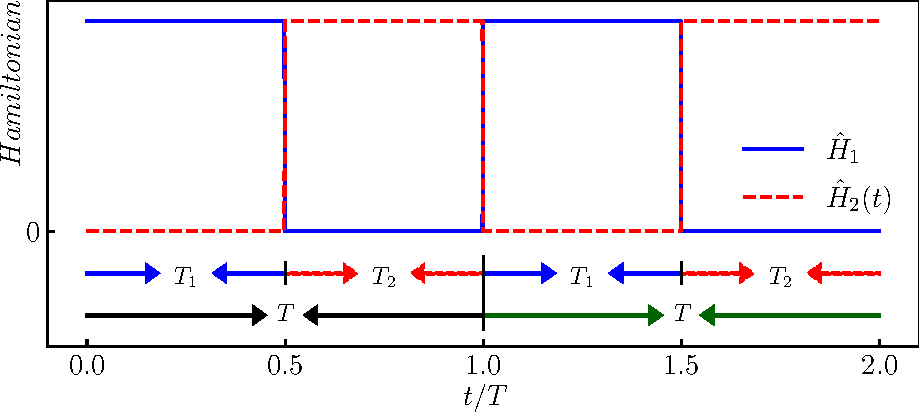
\includegraphics[width=10cm]{figure1.pdf}
    \end{center}
    \caption{Pictorial realization of the temporal progression of the Hamiltonian in Eq.~\eqref{eq:cleanham}. The modulating pulses are set in such a way that the spin-flipping Hamiltonian $\hat{H_1}$, depicted as Eq.~\eqref{eq:sysham1}, acts during the $T_1-$cycle (blue curve), and the harmonic drive as well as the interactions, depicted as $\hat{H_2}(t)$ in Eq.~\eqref{eq:sysham2}, acts during the $T_2-$cycle(red dashed curve).}
    \label{Fig:time_distribution}
\end{figure}	
and $\hat{\sigma}^{\mu=x,y,z}_i$ are the Pauli matrices at $i$-th site.  Henceforth, we shall simplify our analysis by assuming that the pulse waves modulating these Hamiltonians have a $50 \%$ duty-cycle, \textit{i.e.} $T_1=T_2=T/2$.  The Hamiltonian $\hat{H}_1$ in equation~\eqref{eq:sysham1} represents a transverse field that can perform spin-flips on spins. To realize the DTC phase on the chain, we set an \textit{ideal value} of this field at $g=\pi/T$. Now, we divide the chain into two physical regions denoted by $A$ and $B$, based on two relative deviations $\epsilon_{A/B}\in[0,1]$ of the field from this ideal value. Thus, these deviation parameters are \textit{rotational errors} for the two regions, and play an essential role in differentiating between the two regions~\footnote{For instance, when $\epsilon_A \sim 0$ and $\epsilon_B \sim 1$, the field in region-A cause imperfect spin-flips, while that in region-B do not flip most spins.}.

The Hamiltonian $\hat{H}_2$ in equation\eqref{eq:sysham2} represents a standard long-range spin-chain in $1-$dimension. The first term models the interaction between two sites $(i>j)$ with a coupling strength $J_{ij}$, assumed to follow a power-law decay $J_{ij}={J_0}/{|i-j|^\beta}$. We have adapted Buyskikh's benchmarking ~\cite{buyskikh_entanglement_2016} to classify the scaling of the spin-spin interaction by varying $\beta$. According to this classification, when $\beta\in\left[0,1\right)$, the interaction is classified as \textit{long-range}, with $\beta=0$ called the \textit{all-to-all} interaction; the range $\beta\in \left(1,2\right)$, as the \textit{ intermediate range} interaction; the range $\beta > 2$ as the \textit{ short-range} interaction, with $\beta= \infty$ called the \textit{ nearest-neighbor} interaction. The second term in $\hat{H}_2$ is a continuous transverse time-periodic drive $\displaystyle \hat{H}_D=\hbar h_D \sum_i\hat{\sigma}^z_i$, where $\displaystyle h_D = -h\sin{(\omega t)}$, and $h,\omega$ are the amplitude and frequency (respectively) of the drive. We have considered $\omega$ to be high enough such that $\omega\gg J_0$. 	Experimentally, this can be accomplished using external high-frequency drives whose time scales are significantly shorter than the relaxation rate due to the interactions in $\hat{H}_2$.~\cite{choi_observation_2017,zhang_observation_2017,Cirac_1995,Blatt_2012}. At specific values of $h$ and $\omega$, our model shows a dynamical state that facilitates the manifestation of CDT/DL, which prevents the system from rapid thermalization. We will elaborate on this in section~\ref{sec:level2}. The final term in both $\hat{H}_{1,2}$, in equations~\eqref{eq:sysham1}, and~\eqref{eq:sysham2}, is $\displaystyle \hat{V}(\hat{\sigma}^{\gamma}) \equiv\gamma  \sum_{i=1}^{N} (\hat{\sigma}^x_i + \hat{\sigma}^y_i)$. It serves as a controlled additional static field that operates on the entire spin chain in the $x$ and $y$ spin axes, respectively.  This term can also be interpreted as a static magnetic imperfection that is modulated by a parameter $\gamma$. We have chosen to ignore this by default, and reintroduce it in section \ref{sec:level4} in order to investigate the robustness of the chimera against such imperfections.
\begin{figure}[t!]
    \centering
    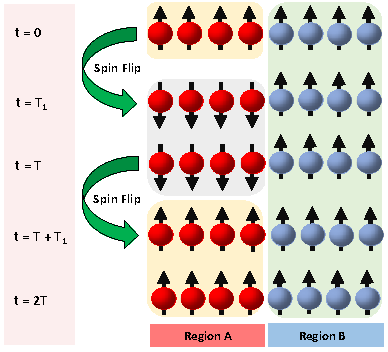
\includegraphics[width=7.cm]{figure2.pdf}
    \caption{Spin-flips that arise in the spin-$1/2$ chain due to the dynamics described in Eqs.~\ref{eq:sysham1} and~\ref{eq:sysham2}, where the system is broken into two regions, $A$ (left panels) and $B$ (right panels). Snapshots at times $t=0, T_1, T, T+T_1 $ and $t=2T$ are represented from the top to bottom panels, respectively. The spins in the region $B$ remain unchanged for all time. In the region $A$, the spins are flipped in $T_1$ and preserved by CDT/DL during the $T_2-$cycle until $t=T_1+T_2=T$. In the next $T_1-$cycle, they are flipped back and preserved again by CDT/DL until $t=2T$. Thus, the region $A$ has a \textit{period-doubling} response from $t=0$ to $t=2T$.}
    \label{Fig:spinflip}
\end{figure}
	
	We populate the spins in a fully polarized product state of up-spins, as depicted in the top panel of figure~\ref{Fig:spinflip}. During the $T_1-$cycle of the pulses,  the spins in region A \textit{ideally} undergo a \textit{spin-flip} resulting in a spin-down orientation, while the spins situated within region B, remain ideally unaltered. If the dynamics in the $T_2-$cycle of the pulses remains localized by CDT/DL, this state of affairs continues to time $t=T$, as depicted in the next lower panel of figure~\ref{Fig:spinflip}. The localization ensures that each of the spins of the system is independent of each other, preventing any growth of correlations or entanglement between them during this cycle. Now, when the $T_1-$cycle repeats, the spins in region A are flipped back, thereby restoring the spin chain to its initial spin orientation. The dynamics remains localized during the next $T_2-$cycle due to CDT/DL. Thus, when the system is driven up to the next time period $2T$, a spin magnetization \textit{period doubling}~\cite{rovny_31mathrmp_2018, Pan2020}, or \textit{half frequency subharmonic} response is expected. 
	
\section{\label{sec:level2} Interacting Dynamical Localization}

Before investigating the chimera order in our model, we explain how the Hamiltonian $\hat{H}_2$ in equation~\eqref{eq:sysham2} exhibits CDT/DL by analytically solving for the dynamics during all $T_2-$cycles. During these times,  the entire spin system is driven by a sinusoidal transverse periodic drive $\hat{H}_D$.
	
Let us employ the \textit{moving frame method}~\cite{haldar_dynamical_2021}, where a unitary transformation is performed to the instantaneous rest frame of the rotation representing the drive. The transformation on the state yields $\ket{\psi(t)}_{mov} = \hat{U}^\dagger(t_0,t) \ket{\psi(t)}$, where 
\begin{equation}
    \hat{U}(t_0,t) \equiv \mathcal{T} e^{-\frac{i}{\hbar}\int_{t_0}^{t} dt' \hat{H}_D}.
    \label{eq:rot1}
\end{equation}
During the first $T_2-$cycle, $t \in{\Big[\frac{T}{2}, T \Big]}$. Thus,
\begin{equation}
    \hat{U}\left(T/2,t\right) = \exp \Bigg[-\frac{i}{\hbar}\int_{T/2}^{t+T/2} (-h \sin(\omega t'))dt'\hbar\sum_i\hat{\sigma}^z_i\Bigg]
    = \prod_{i} \exp\Big[-i \hat{\sigma}^z_i\zeta(t))\Big],
\end{equation}
where, $\displaystyle{
    \zeta (t) = h\int_{T/2}^{T/2+t}  \Big[-\sin(\omega t')dt'\Big]=  \frac{h}{\omega}\Big[1-\cos(\omega t)\Big]}$.		
Now, in this `rotating frame', the Hamiltonian transforms to (see~\ref{sec:AppendixA} for details),
\begin{align}
    \hat{H}^{mov}(t) &= \hat{U}^\dagger \hat{H}_2(t) \hat{U}- i \hat{U}^\dagger \partial_t \hat{U},\nonumber\\
    &=\hbar\sum_{ij}J_{ij}\Big\{\hat{\sigma}^y_i\cos{\big[2\zeta(t)\big]}-\hat{\sigma}^x_i\sin{\big[2\zeta(t)\big]}\Big\}\Big\{\hat{\sigma}^y_j\cos{\big[2\zeta(t)\big]}-\hat{\sigma}^x_j\sin{\big[2\zeta(t)\big]}\Big\},
    \label{eq:movham}
\end{align}
where, in the last step, we have employed the Baker-Campbell-Hausdorff formula. Next, we decompose the moving frame Hamiltonian into its Fourier modes and introduce the Rotating Wave Approximation (RWA), which, in the high-frequency limit, approximates the Fourier modes with their coarse-grained values over long times. This allows us to average out all but the zeroth Fourier mode (see~\ref{sec:AppendixA} for details). This yields
\begin{multline}
\hat{H}^{mov}\approx \hat{H}^{_{RWA}} = \frac{\hbar}{2}\sum_{ij} J_{ij} \hat{\sigma}^y_i\hat{\sigma}^y_j\Bigg\{\left[1+\cos(\frac{4h}{\omega})\mathcal{J}_0\left(\frac{4h}{\omega}\right)\right] \\
+ \hat{\sigma}^x_i\hat{\sigma}^x_j \left[1-\cos(\frac{4h}{\omega})\mathcal{J}_0\left(\frac{4h}{\omega}\right)\right]
+ \left(\hat{\sigma}^x_i\hat{\sigma}^y_j+\hat{\sigma}^y_i\hat{\sigma}^x_j\right)\sin(\frac{4h}{\omega})\mathcal{J}_0\left(\frac{4h}{\omega}\right) \Bigg\}.
\label{eq:movham1}
\end{multline}
Now, if the drive parameters $h$ and $\omega$  are engineered in such a way that the ratio ${4h}/{\omega}$ lies at one of the higher roots of $\mathcal{J}_0$~\footnote{This can be achieved when $\omega \gg J_0$ by ensuring that $h\gg J_0$.}, it is possible to nullify the dynamics of $\hat{H}_2$ during all $T_2-$cycles, thus inducing localization in the system. We have supported this result by numerical simulations, detailed in section~\ref{sec:level42},where, $\hat{\sigma}^z$ is detected as an approximate integral invariant ~\cite{Keser2016,Dodonov1978}. 

\section{\label{sec:level3}Coexistence of DTC \& DMBL}	
The underlying dynamics of the periodic Hamiltonian of the chimera model outlined in section~\ref{sec:mdl_n_dynam} can be understood by employing the Floquet theory (FT). FT allows us to examine the dynamics at the stroboscopic times, namely, at integer multiples of the time period $T$. The effective Floquet Hamiltonian($H^{\mathrm{eff}}$) for the proposed spin-system that undergoes two periods can be written as follows:
\begin{multline}
    H^{\mathrm{eff}} \approx\frac{\hbar}{2} \sum_{l,m\in A}J_{lm}\hat{\sigma}_l^y\hat{\sigma}_m^y +\frac{\hbar \epsilon_A \pi}{4} \sum_{\substack{l,m\in A\\l\neq m}} J_{lm}\hat{\sigma}^z_l\hat{\sigma}^y_m + \frac{\hbar}{2}\sum_{l,m\in B}J_{lm}\hat{\sigma}_l^y \hat{\sigma}_m^y + \frac{h\hbar}{\pi}\sum_{m \in B}\hat{\sigma}^z_m \\ -\frac{\hbar \pi \epsilon_A}{4T}\sum_{l\in A}\Bigg\{\hat{\sigma}^x_l \bigg[\cos(\hat{\theta}_l)\cos(\frac{4h}{\omega})+1 \bigg] + \hat{\sigma}^y_l \cos(\hat{\theta}_l)\sin(\frac{4h}{\omega})-\hat{\sigma}^z_l \sin(\hat{\theta}_l)\Bigg\}.
    \label{eq:floq_eff3}
\end{multline}
Here, $\displaystyle \hat{\theta}_l \equiv 2 \Big(\sum_{m \in B}J_{lm}\hat{\sigma}^y_m \frac{T}{2} \Big)$ denotes a rotation acting on $\hat{\sigma}^y_l$, the local $y-$spin\footnote{See~\ref{sec:AppendixB} for details.}. 
To examine the influence of rotational error on the chimera order, let us begin by considering the scenario where $\epsilon_A=0$. In this situation, the effective Hamiltonian $H^\mathrm{eff}$ in equation~\eqref{eq:floq_eff3}  decouples into terms that live separately in regions A and B, \textit{i.e.},
\begin{equation}
    H^{\mathrm{eff}}_{\epsilon_A=0} =  \frac{\hbar}{2}\Bigg( \sum_{l,m\in A} J_{lm} \hat{\sigma}^y_l\hat{\sigma}^y_m +\sum_{l,m\in B} J_{lm} \hat{\sigma}^y_l\hat{\sigma}^y_m\\+\frac{2h }{\pi}\sum_{m \in B}\hat{\sigma}^z_m\Bigg).
\end{equation}
	
In such a case, the quantum dynamics of the two regions exhibit mutual independence when the system is first prepared in a state that can be factorized as a product of states in the invariant subspaces of regions A and B, respectively. Since we still have a significant degree of flexibility in selecting the driving parameters, it is possible to configure them in such a way as to induce DMBL in the region $B$, while preserving a stable DTC in the region $A$. Let us now increase the parameter $\epsilon_A$ while maintaining a sufficiently high frequency for the drive, so that it is possible to disregard the term $\hat{\theta}_l \approx 0$ due to condition $T<<\hbar/J_0$. Under these circumstances, the strength of the coupling between two regions is significantly influenced by the ratio $4h/\omega$. This dependence is characterized by the amplitudes $(1+\cos(4h/\omega))$ and $\sin(4h/\omega)$, which exhibit non-monotonic behavior. Specifically, when $4h/\omega$ takes the form of $(2n+1)\pi$, where $n$ is a non-negative integer, the decoupling of regions A and B occurs again, regardless of the value of $\epsilon_A$ being nonzero.
\begin{figure}[h!]
    \centering
    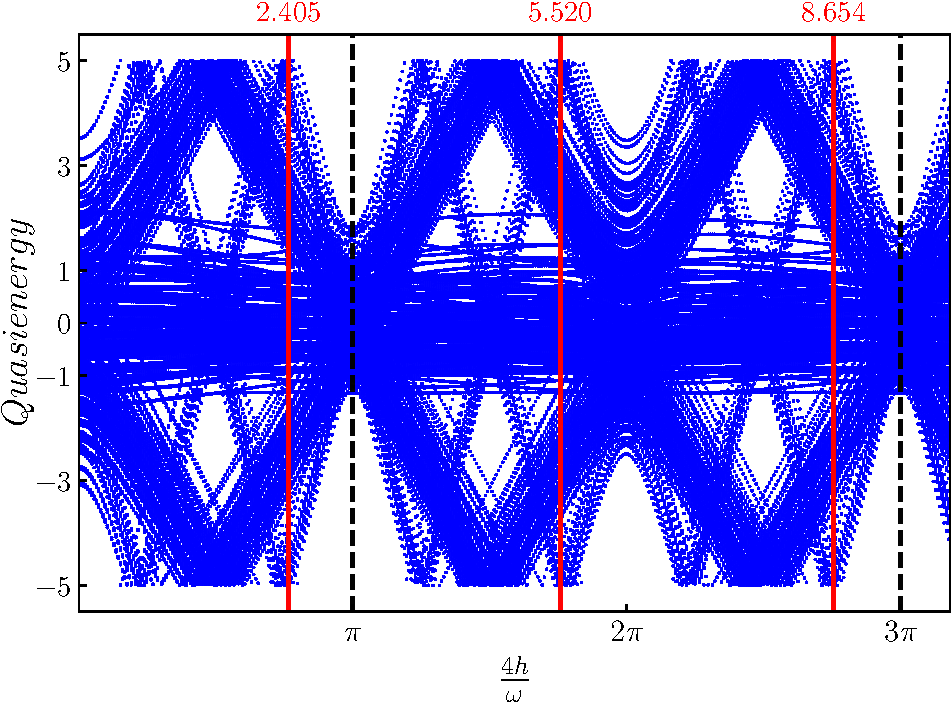
\includegraphics[width=10cm]{figure3.pdf}
    \caption{Floquet quasi-energies of the driven spin-chain,  estimated by numerically diagonalizing $H^{\rm eff}$ in equation~\eqref{eq:floq_eff3} at 2T for the one dimensional spin-$1/2$ chain. In this simulation, the number of spins $N=8$ and the strong coupling $J_0=0.2/T$ is considered. The quasi-energies are plotted for different values of $h,\omega$, the amplitude, and frequency of the periodic drive, respectively.  The x-coordinate plots ${4h}/{\omega}$, where $\omega( = 20)$ is kept constant and only $h$ is changed, and the y-coordinate plots the corresponding quasi-energies. Level repulsion is minimum when ${4h}/{\omega} = (2n+1)\pi$, $n\in \mathbb{N}_0$. The first such point is shown as a vertical black dashed line. Solid red lines indicate the roots of the zeroth-order Bessel function $\mathcal{J}_0(4h/\omega)$.}
    \label{Fig:quasienergy_new}
\end{figure}	

\begin{figure*}[t!]
    \centering
    \hspace{2cm}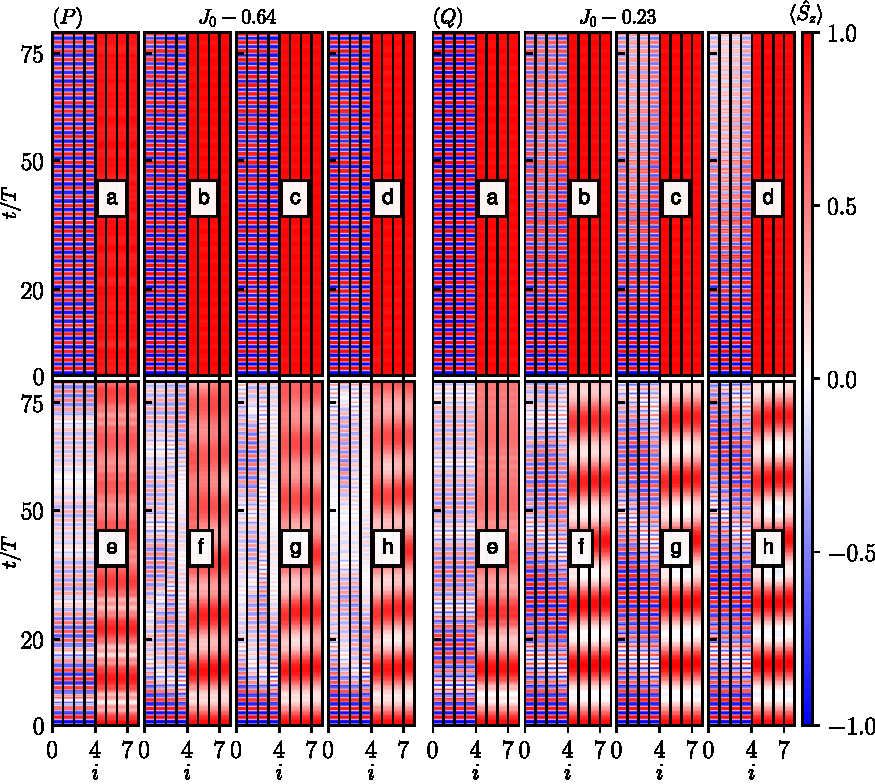
\includegraphics[width=13.5cm]{figure4.pdf}
    \caption{The time evolution of local magnetization for each spin at region A (i=0,1,2,3) and region B (i=4,5,6,7) is plotted for $N=8$ spins in a periodically driven one-dimensional spin chain, starting from a fully polarized spin state, with drive frequency $\omega=20$. The spin rotation error $\epsilon_A = 0.03$ and $\epsilon_B = 0.9$, and $g=\pi/T$, where $T=2\pi/\omega$ is the time period of the drive.  In all two panels, different ranges of spin-interactions such as long-range($\beta=0$), intermediate range($\beta=1.5$), short range($\beta=2.5$), and nearest neighbor range($\beta=\infty$), are chosen and plotted, respectively, from left to right, namely (a, b, c, d) in the top row and (e, f, g, h) in the bottom row of each panel. The results of the time evolution for the weak spin coupling ($J_0 = 0.072/T$) are shown in the left panel (P) and the strong spin coupling ($J_0 = 0.2/T$) in the right panel (Q). The top panels of P \& Q show plots where the drive amplitude $h$ is chosen so that the system lies at the CDT / DL point, and the bottom panels show the results away from that CDT/DL point.}
    \label{Fig:strong_weak_ea}
\end{figure*}

We have utilized numerical estimations of eigenvalues to represent the effective Hamiltonian $H^{\rm eff}$. These are connected to the \textit{ Floquet quasienergies} of the driven spin chain, given by the eigenvalues of the time-dependent observable $\hat{H}(t)-i\hbar\pdv*{}{t}$ evaluated at $t=2T$. The numerical diagonalization of the effective Hamiltonian $H^{\rm eff}$ has been performed for a system of $N=8$ spins. The resulting quasi-energies have been displayed as a function of ($4h/\omega$). The results are depicted in figure~\ref{Fig:quasienergy_new}. The quasi-energy distribution displays a consistent pattern that is confined to the Floquet-Brillouin zone, namely the interval of $[-\frac{\pi}{2T}, \frac{\pi}{2T}]$, a consequence of Floquet's Theorem~\cite{dutta2014}. It is evident that the minimum repulsion between the quasi-energies occurs when the parameter $4h/\omega$ is an odd integer multiple of $\pi$. This result offers empirical evidence that is consistent with the theoretical assertions presented earlier in this section on the decoupling of region A and B, even in the cases where $\epsilon_A \neq 0$. Nevertheless, the CDT/DL condition in region-B necessitates that $4h/\omega$ lie on one of the higher roots of the Bessel function. This condition retains the existing coupling between regions A and B for a nonzero $\epsilon_A$. Therefore, $\epsilon_A$ is the key system parameter to control the coupling between the two regions of our proposed model. 	
	
We now present visuals of the local magnetization, denoted as $\expval{\hat{S}^z_i (t)}$, which is equivalent to the expectation value of the operator $\hat{\sigma}^z_i$ with respect to the state $\ket{\Psi(t)}$, for all sites $i$ in the spin-chain. The data mentioned above have been obtained using numerical simulations of Schr\"odinger dynamics, represented by the equation $\hat{H}(t)\ket{\Psi(t)}= i \hbar \pdv*{\ket{\Psi(t)}}{t}$. This equation describes the behavior of the quantum many-body state $\ket{\Psi(t)}$. Simulations were carried out using QuTiP, a Python-based Quantum Toolbox~\cite{Johansson2013}. The simulations were performed over an extended duration (up to $t = 80T$, with $\hbar$ normalized to unity) and over various ranges of power law interactions ($\beta = 0,1.5,2.5,\infty$). Furthermore, simulations were carried out for weak and strong interaction amplitudes ($J_0 = 0.072/T$ and $J_0 = 0.2/T$ respectively), which are similar to the parameters selected by in previous study~\cite{sakurai_phys_nodate,zhang_observation_2017}. To assess the durability of this chimera, we set the rotational error values as $\epsilon_A = 0.03$ and $\epsilon_B = 0.9$. Furthermore, to observe the emergence of the chimera state in our model, we manipulate the periodic drive in $\hat{H}_2(t)$ by setting a high frequency $\omega=20$ for two different scenarios: one where the parameter $4h/\omega$ is located at a \sout{higher} root \sout{(third root)} of the Bessel function $\mathcal{J}_0(4h/\omega)$, specifically at the CDT/DL point, and another where $4h/\omega$  does not lie at any roots of $\mathcal{J}_0$.
	
As illustrated in figure~\ref{Fig:strong_weak_ea}, the local magnetization exhibits the breaking of discrete time translational symmetry, manifesting a DTC phase in region A at the CDT/DL point, under the condition of strong spin-spin coupling. Simultaneously, region B exhibits localized dynamics. As a result, the coexistence of the DTC and DMBL phases is observed in regions A and B, respectively, leading to the formation of a chimera state. Conversely, it is evident that the system dynamics demonstrate instability upon deviation from the CDT/DL point, irrespective of the particular values of coupling strength($J_0$) that have been chosen. In a similar vein, it can be noted that weak interactions demonstrate the presence of a stable chimera state when they possess a range that encompasses all spins ($\beta=0$). However, when considering intermediate ($\beta = 1.5$), short ($\beta = 2.5$), and nearest-neighbor range interactions ($\beta = \infty$), the DTC melts rapidly inside region A, typically occurring within $20$ cycles of the drive. This result is consistent with the findings of previously published work~\cite{sakurai_phys_nodate}.
	
The stability of this DTC phase exhibits notable disparities between strong and weak-coupling interactions. At the CDT/DL point, it is seen that the DTC phase exhibits enhanced stability in the presence of strong coupling compared to weak coupling, specifically for interactions that are not long-range in nature. The phenomenon of stable DTC is observed in long-range spin chains, regardless of the strength of spin interactions. Therefore, it is feasible to see the emergence of a chimera state consisting of two separate phases of matter, specifically a time crystal and a localized ferromagnet, simultaneously in a spin-chain system. This phenomenon can occur in typical experimental settings, with long-range interactions being the most suitable candidate.
\begin{figure}[t!]
\centering
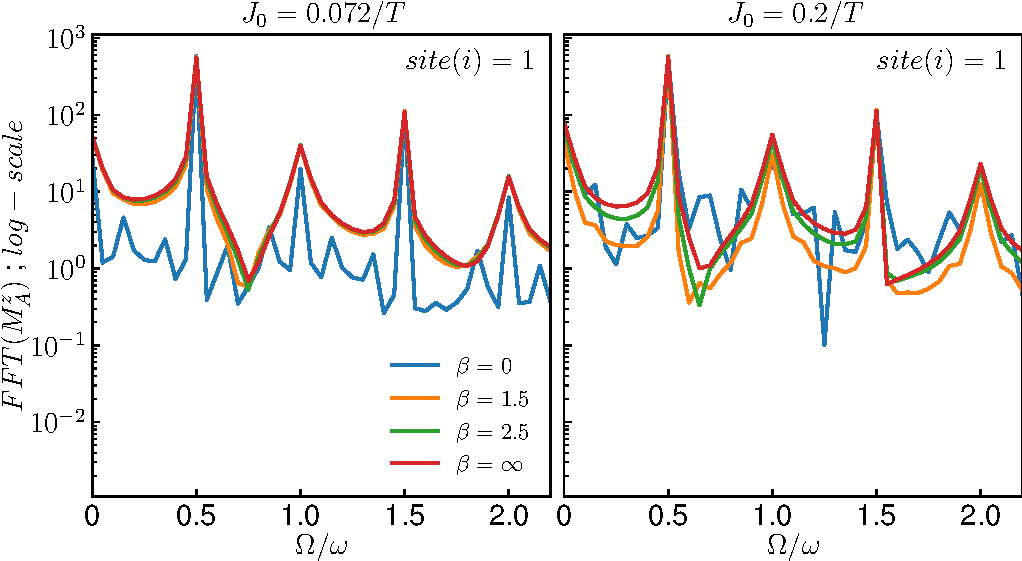
\includegraphics[width=10.cm]{figure5.pdf}
\caption{Fast Fourier Transforms(FFT) of the local magnetization at site $i=1$ in region A of the spin-chain for weak coupling ($J_0 = 0.072/T$, left panel) and strong coupling ($J_0 = 0.2/T$, right panel) for different values of $\beta$ as indicated in the legend. The amplitude $h$ is adjusted so that the system is at the smallest CDT/DL point. All other parameters are the same as those in Fig.~\ref{Fig:strong_weak_ea}. The peaks at half-integer multiples of $\omega$ denote subharmonic responses in region A that result in stable DTC.}
\label{Fig:sz_single}
\end{figure}
	
The suitability of long-range interactions is examined by analyzing the dynamics in frequency space (with the frequency variable denoted by $\Omega$) by applying a Fast Fourier Transform (FFT) on the local magnetism at a specific spin site $(i=1)$ in region A. Numerical FFT algorithms provided by the NumPy library were utilized to achieve this task~\cite{harris2020array}. The results are visually presented in figure\ref{Fig:sz_single}.  The frequency $\Omega$ in the x-coordinate has been scaled relative to the driving frequency $\omega$. The subharmonic response at $\Omega=\omega/2$ can be detected by observing the peaks at half-integer multiples of $\omega$. This observation serves as confirmation of the onset of discrete TTSB throughout all selected spin-interaction ranges. The stability of the resulting DTC will be influenced by the contributions originating from the underlying continuum of frequencies. When $\beta$ approaches zero, the continuum exhibits a higher degree of submissiveness toward subharmonic peaks compared to higher values. This distinction is especially noticeable under conditions of weak coupling. Therefore, in the context of a DTC phase of matter, it is advantageous to consider long-range interactions rather than short-range interactions when selecting potential candidates. The present analysis is consistent with the numerical results shown in figure\ref{Fig:strong_weak_ea}, where each individual spin interaction type provides evidence of a reliable DTC.	
\begin{figure}[t!]
\centering
\hspace{1.5cm}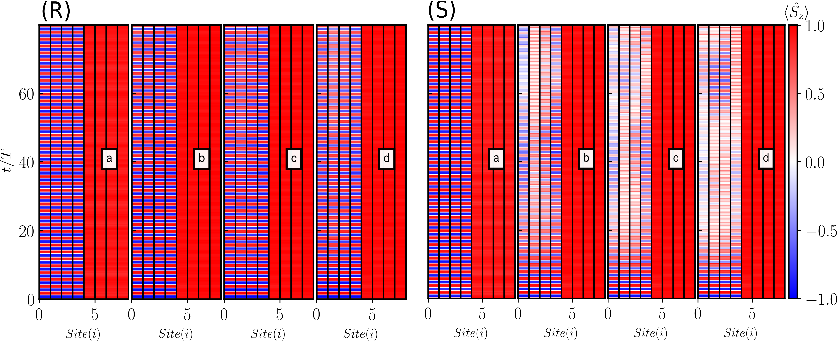
\includegraphics[width=13.5cm]{figure6.pdf}
\caption{The time evolution of local magnetization for each spin at region A (Site(i)=0,1,2,3) and region B (Site(i)=4,5,6,7) is plotted for $N=8$ spins in a periodically driven one-dimensional spin chain, starting from a fully polarized spin state, with drive frequency $\omega=20$. The strong spin-spin coupling $J_0 = 0.2/T$, spin rotation error $\epsilon_B = 0.9$ and $g=\pi/T$, where $T=2\pi/\omega$ is the time period of the drive.  Different ranges of spin-interactions such as long-range($\beta=0$), intermediate range($\beta=1.5$), short range($\beta=2.5$), and nearest neighbor range($\beta=\infty$), are chosen and plotted  for $\epsilon_A =0.05$(R-panel) and $\epsilon_A =0.1$(S-panel), respectively, from left to right, namely (a, b, c, d) in each panel.}
\label{Fig:ea}
\end{figure}

Furthermore, we have conducted an analysis on the resilience of the DTC in the presence of larger rotational errors \red{($\epsilon_A$)}. The simulation results are presented in figure~\ref{Fig:ea}. In the present simulations, we examine two different values for the parameter $\epsilon_A$, namely $\epsilon_A = 0.05$ and $\epsilon_A = 0.1$, while maintaining a constant value of $\epsilon_B$ at $0.9$. In this study, we investigate various ranges of interactions, denoted by the parameter $\beta$, which assumes the values of $0.0, 1.5, 2.5$ and infinity. The aforementioned investigations are carried out at a CDT/DL point under strong coupling, $J_0 = 0.2/T$.  A steady DTC was observed for all interaction ranges when the value of $\epsilon_A$ was set to $0.05$. The stability of the DTC is maintained for higher values of $\epsilon_A$, that is, when $\epsilon_A = 0.1$ only when all-to-all interactions ($\beta=0$) in considered. However, in the case of spin-spin interactions with other ranges, the DTC  diminishes rapidly. This finding provides further evidence in favor of the proposal that long-range interactions are the most advantageous for the development of a DTC-MBL chimera.
\begin{figure}[t!]
	\centering
	\hspace{2cm}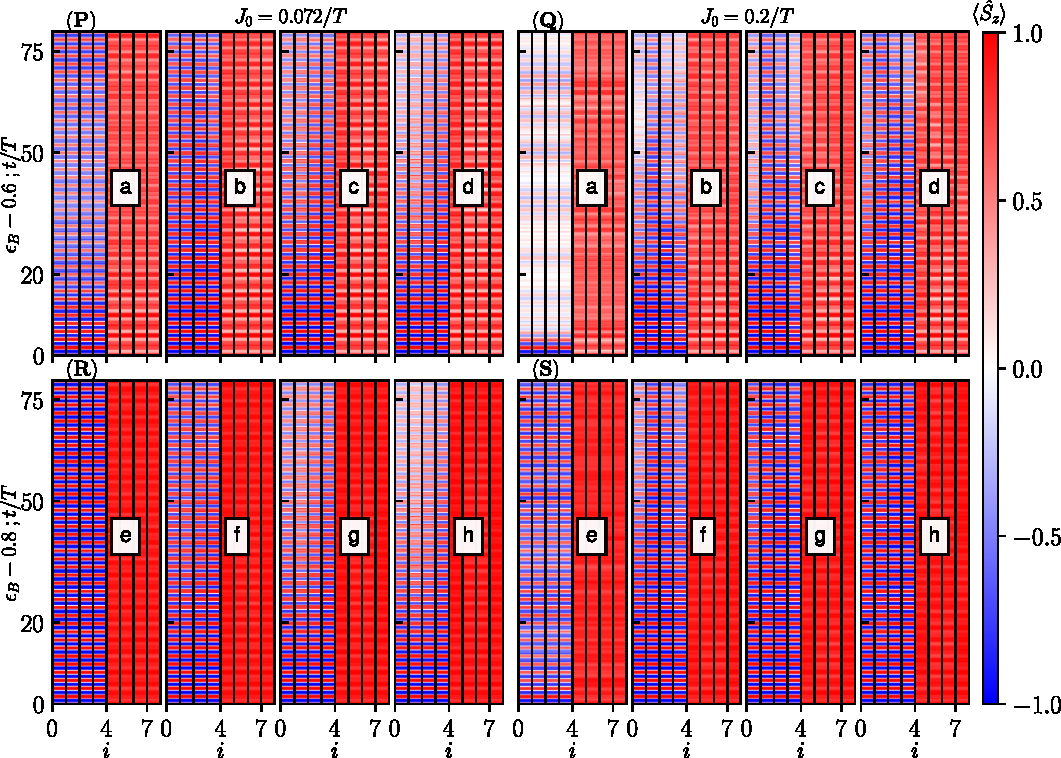
\includegraphics[width=13.5cm]{figure7.pdf}
	\caption{\red{The time evolution of local magnetization for each spin at region A (i=0,1,2,3) and region B (i=4,5,6,7) is plotted for $N=8$ spins in a periodically driven one-dimensional spin-1/2 chain, starting from a fully polarized spin state. We have considered the drive frequency $\omega=20$ and amplitude corresponding to CDT/DL point. The strong spin-spin coupling $J_0 = 0.2/T$ (panels Q \& R) and weak spin-spin coupling $J_0 = 0.072/T$ (panels P \& R),  spin rotation error $\epsilon_A = 0.03$ and $g=\pi/T$, where $T=2\pi/\omega$ is the time period of the drive. The upper panels (P \& Q) denote plots for $\epsilon_B=0.6$ and lower panels (R \& S) denote plots for $\epsilon_B=0.8$. Different ranges of spin interactions such as long-range($\beta=0$), intermediate range($\beta=1.5$), short range($\beta=2.5$), and nearest neighbor range($\beta=\infty$), are chosen respectively, from left to right, namely (a, b, c, d) in each panel.}}
	\label{Fig:eb}
\end{figure}
\red{This observation holds true for the cases where the spin rotational error $\epsilon_B$ is large ($\sim 0.9$), while $\epsilon_A$ remains relatively small ($\le 0.1$).}

\red{To investigate the impact of $\epsilon_B$ on the emergence of a chimeralike state, we have considered the spin-1/2 chain with all sites initially populated with up-polarized spins. We have considered strong ($J_0 = 0.2/T$) and weak ($J_0 = 0.072/T$) spin-coupling strength with drive frequency $\omega = 20$ and an amplitude corresponding to a CDT/DL point, maintaining constant $\epsilon_A=0.03$. We have obtained numerical results as well as a plot showing the change in local magnetization over time in figure~\ref{Fig:eb} for different spin-spin interaction ranges at each site (i) for two values of $\epsilon_B$ which are $\epsilon_B = 0.6$ and $\epsilon_B = 0.8$. For both of the $\epsilon_B$'s values, the DMBL phase in region B is found to lack of its stability in course of time, although the drive parameters are kept at CDT/DL point. The instability in DMBL increases as $\epsilon_B$ decreases. The DTC phase in region A melts for all cases of $\epsilon_B$ and interaction ranges. However, the rate of melting of DTC at different sites (i=0,1,2,3) varies depending on the values of $\epsilon_B$ and interaction ranges. For a particular $\epsilon_B$ (say $\epsilon_B=0.8$), each of the spins in region A exhibits almost similar dynamics over time only for all-to-all interaction. However, at other shorter interaction ranges, they posses distinct dynamics. The spins far away from the bipartite junction melts its DTC phase faster than the spins closer to the junction. Their rate of melting of DTC phase is faster in case of weak coupling strength in comparison to strong coupling strength. However, in case of all-to-all interaction, the DTC-melting behavior is opposite to that of shorter range interactions; the DTC phase melts slower in weak coupling than the strong coupling. In case of smaller $\epsilon_B=0.6$ we have observed that for each of the cases of coupling strength and interaction ranges, the rate of melting is faster than that of $\epsilon_B=0.8$.}

\red{ In general, each of the spins in region A interacts equally with the spins in region B over the course of time for the all-to-all interaction range ($\beta=0$). This results in the melting of the DTC phase occurs at equal rates for particular spin rotational error for all-to-all spin interaction. For shorter interaction ranges, the spins of regions A, which are away from the bipartite junction, achieve less interactions with DMBL in region B, depending on the length of the interaction. This results in faster local melting in the DTC phase at the far-away spins from the junction than the spins nearby. Thus, the rate of melting of DTC at each site in region A increases as the length of the spin-spin interaction decreases. This corroborates the better stability of chimeralike order in all-to-all interactions, and when $\beta$ increases, stability decays. For higher coupling strengths, the rate of interaction increases. This explains why the chimeralike state melts faster in strong coupling and all-to-all interactions than in weaker ones. Additionally, in shorter-range interactions, at strong coupling strength due to the increase in interaction between spins in DTC and DMBL phases, the chimeralike state melts at slower rate, comparing to the weak coupling strength. Thus, at a smaller rotational error $\epsilon_B$, the DTC-DMBL chimeralike order is not sustainable for a longer time period.}

\red{ Therefore, we have considered a small $\epsilon_B = 0.3$ and a high $\epsilon_B = 0.9$ value to sustain a stable chimeralike state throughout the manuscript. Also, a strong coupling is preferable to investigate the short time dynamics of the DTC-DMBL chimeralike order.}\todo{\small MR: Check if this addendum can be shorten and more affluent.}

\section{\label{sec:level4} Stability of the chimera phase}
In this section, we investigate the stability of the chimera\red{like} phase in various regions of the complex parameter space. We observe simulations run for both strong and weak coupling with a wide variety of interaction ranges. The physical phenomena of interest involve the tunneling of any quantum information between the DTC and the DMBL regions that would serve to melt the DTC, and can be profiled by looking at the regional magnetization as well as the entanglement entropy between the regions, as functions of time. Finally, we investigate the robustness of the chimera against external static fields.
\subsection{\label{sec:level42} Regional Magnetization}
\begin{figure}[t]
	\centering
	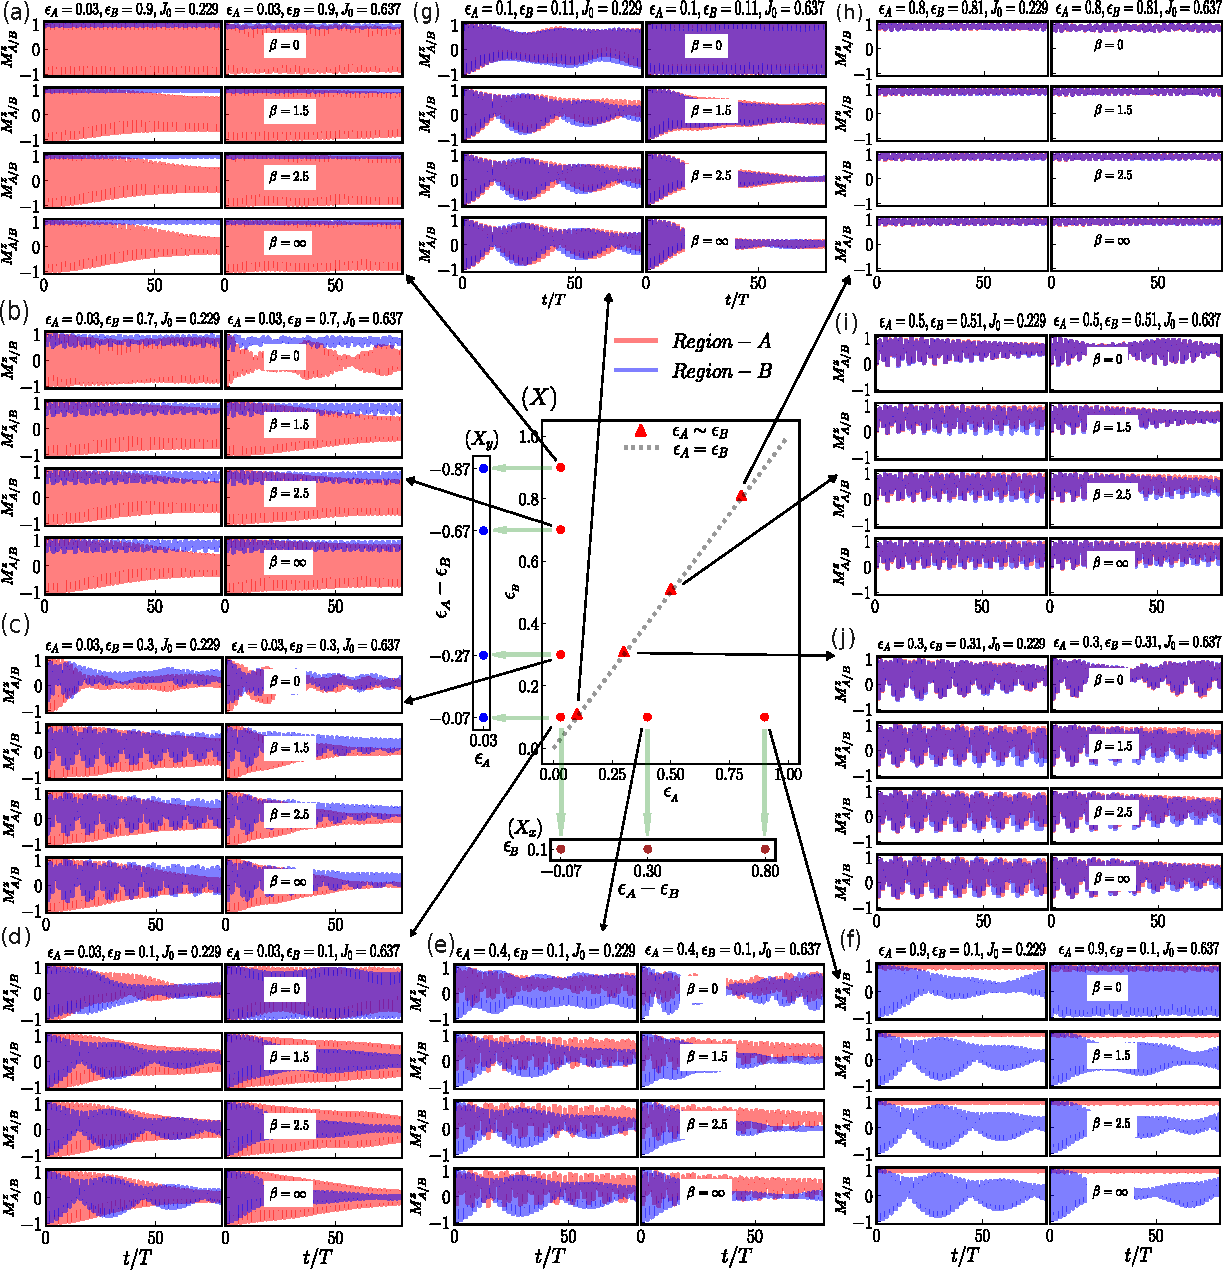
\includegraphics[width = 15.0cm]{figure8.pdf}
	\caption{\red{Temporal variation in regional magnetization $M^z_{A/B}$ of the spin-1/2 chain upto 80T for various spin rotational errors ($\epsilon_{_{A,B}}$) in different panels for  several ranges of spin interactions (characterized by $\beta$). The time period (T) is fixed by setting the drive parameters $\omega=20$ and $h$ to the CDT/DL point, \textit{i.e.} one of the root of $\mathcal{J}_0(4h/\omega)$. The central panel-X elucidates the selection of $\epsilon_{A,B}$'s and points out corresponding panel-plots. We have considered $\epsilon_A = 0.03$ and varied $\epsilon_B(= 0.1, 0.3, 0.7,0.9$) and corresponding plots are in left panels namely `d',`c',`b',`a' respectively.  For the constant $\epsilon_B = 0.1$ and varying $\epsilon_A ( = 0.03, 0.4,0.9$), the corresponding plots are in bottom panels namely `d',`e' and `f' respectively. Furthermore a set of $\epsilon_{A,B}$ which is $ (\epsilon_{A},\epsilon_{B}) = \{(0.1,0.11), (0.3,0.31),(0.5,0.51),(0.8,0.81))\}$ is considered ensuring $\epsilon_A\sim \epsilon_B$ and corresponding plots are in panels namely `g',`j',`i' and `h' respectively. In each cases, weak ($J_0 = 0.229$) and strong ($J_0 = 0.637$) spin coupling  is considered and denoted in left and right side of sub-panels respectively. The differences in selected $\epsilon_{A,B}$'s are plotted for constant $\epsilon_A = 0.03$ in $X_y$ panel and for $\epsilon_B = 0.1$ in $X_x$ panel}.}
	\label{Fig:reg_mag_ea_eb}
\end{figure}
We now examine the regional magnetization of the chimera state, which is given by the expectation value  of the total $z-$spin in a specific region. This can enhance our understanding of the suitability of long-range interactions for the formation of stable time crystals. The expression for the magnetization of regions A and B is $M^z_{A/B}=\frac{2}{N}\sum_{i\in{A/B}}\expval{\hat{\sigma}^z_i(t)}$~\cite{sakurai_phys_nodate}.\red{We have conducted an extensive investigation into various spin rotational errors ($\epsilon_{_{A,B}}$) in order to provide a detailed analysis of the stability of the DTC-DMBL chimeralike order. We have explored different values of rotational error by keeping one of the $\epsilon_{_{A/B}}$ constant and adjusting the other from lower to higher values. In addition, we have adjusted both $\epsilon_A$ and $\epsilon_B$ in such a way that $\epsilon_A \sim \epsilon_B$. We have performed  numerical investigation on the regional magnetization up to 80T. We have  considered various spin-spin interactions, defined by $\beta = 0,1.5,2.5,$ and $\infty$. All spins are considered initially at the spin-up polarized orientation. The drive parameters ($h,\omega$) are set to ensure that the system remains at a CDT/DL point considering frequency $\omega =20$. The numerical data are depicted in figure~\ref{Fig:reg_mag_ea_eb}. In the figure the central primary panel-X elucidates the selection of $\epsilon_A$ and $\epsilon_B$. We have drawn lines connecting the points in $\epsilon_A - \epsilon_B$ space with corresponding $M^z_{A/B}$ plots. }
	
\red{We have considered a constant $\epsilon_{A} =0.03$ and varied $\epsilon_B$ for different values $\epsilon_B(= 0.1, 0.3, 0.7,0.9$) and plotted the temporal variation of $M^z_{A/B}$ in panels, namely `d',`c',`b',`a' respectively. We observe that when $\epsilon_B$ is sufficiently large ($\epsilon_B=0.9$), the DTC-DMBL chimeralike order persists for large time. The DMBL phase is found to be steady for all spin interaction ranges. However, in case of weak coupling ($J_0=0.072/T=0.229$), the DTC phase is found to melt as interaction range shortened ($\beta$ increases). Albeit DTC-melting rate is slower in case of strong coupling ($J_0=0.2/T=0.637$). In case of smaller $\epsilon_B (=0.7,0.3,0.1)$ cases, the stability in DMBL phase decreases as $\epsilon_B$ decreases as well as  the DTC phase melts faster.}

\red{We have obtained $M^z_{A/B}$ data for a set of $\epsilon_A \sim \epsilon_B$ values $(\epsilon_{A},\epsilon_{B}) = \{(0.1,0.11), (0.3,0.31),(0.5,0.51),(0.8,0.81)\}$ (red colored `$\Delta$' points in panel-X) and plotted in panels `g',`j',`i' and `h' respectively. We observe that at small values of $\epsilon_{A,B}$ in both of the regions A and B, the spins experience melting in the DTC phase. When the values of $\epsilon_{A,B}$ increases the DTC phases in both of the region A and B are gradually lost and DMBL phase starts dominating.}

\red{Furthermore in the bottom panels `d',`e',`f' we have considered a constant $\epsilon_{B} = 0.1$ and varied $\epsilon_{A}(=0.03,0.4,0.9)$ in respective panels. When $\epsilon_{A}=0.03~\&~ \epsilon_{B}=0.1$, in panel-d we observe simultaneous melting of DTC phases in region A and B. With further larger $\epsilon_{A}$ values, a transition from a melting-DTC to a stable DMBL is observed in region A in panel-f. Additionally, the stability of DTC phase in region-B increases with increase in $\epsilon_{A}$. Thus at significantly small $\epsilon_{A}$ and large $\epsilon_{B}$ results in a coexisting DTC phase in region B and a DMBL phase in region A, manifesting a chimera like order. For general comprehension we have calculated the relative spin rotational error $\epsilon^r_{A,B} = \epsilon_{A}-\epsilon_{B}$ and plotted in $X_y$ panel, considering constant $\epsilon_{A} = 0.03$ and in $X_x$ panel considering constant $\epsilon_{B} = 0.1$. We observe that only at the extreme values of $\epsilon^r_{A,B}$ which are at small $\epsilon^r_{A,B} \sim -1.0$ in $X_y$ panel or at large $\epsilon^r_{A,B} \sim 1.0$, stable chimeralike order can be obtained and when $\epsilon^r_{A,B}\rightarrow 0$, the chimeralike order vanishes. At extreme small $\epsilon^r_{A,B}$ we observe DTC phase in region A and DMBL in region B. However at extreme large $\epsilon^r_{A,B}$ we observe the opposite; DMBL in region A and DTC in region B. Therefore the selection of rotational errors is a crucial element in engineering and stabilize a DTC-DMBL chimeralike order.} 


\begin{figure}[t]
	\centering
	\hspace{1.5cm}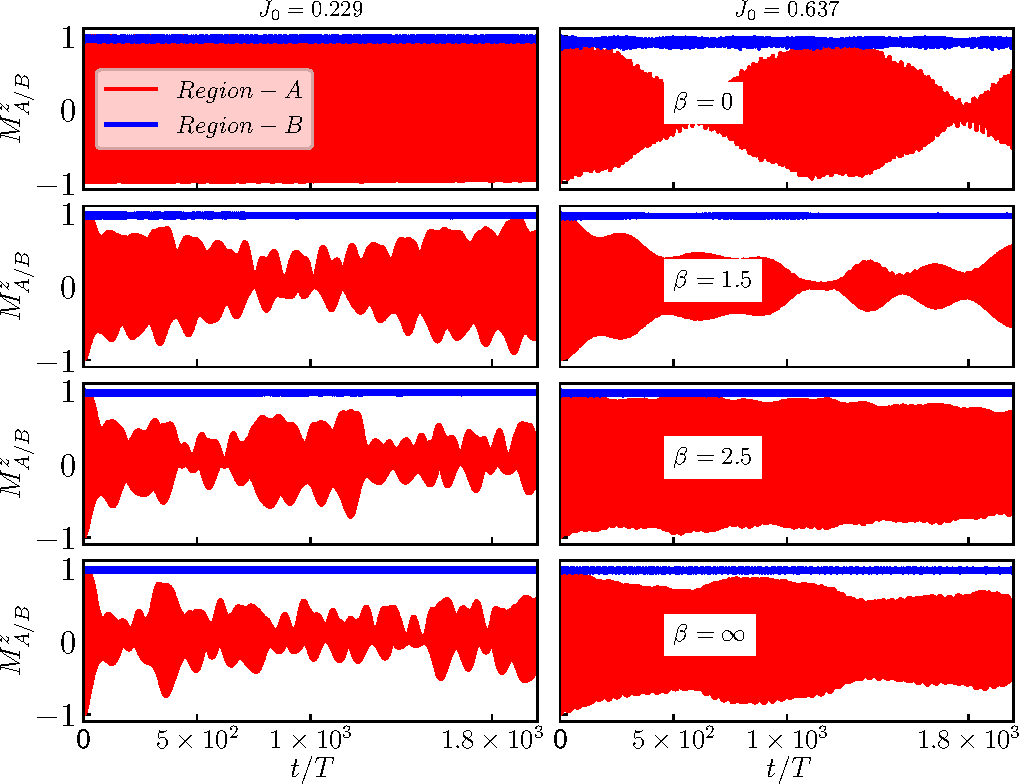
\includegraphics[width = 11cm]{figure9.pdf}
	\caption{Regional magnetization $M^z_{A/B}$ of the spin-chain. The magnetization of regions A (red) and B (blue) is plotted as functions of time $t/T$ \red{upto 2000T} for both weak spin coupling ($J_0=0.072/T$, left panels) and strong spin-coupling ($J_0=0.2/T$, right panels) and different ranges of spin interactions (characterized by $\beta$ as specified in the legends). The time period is fixed by setting the drive parameters $h,\omega$ to the CDT/DL point, \textit{i.e.} the higher root of $\mathcal{J}_0(4h/\omega)$. All other parameters are the same as the simulations visualized in figure~\ref{Fig:strong_weak_ea}.}
	\label{Fig:regiogionalmag}
\end{figure}
We expanded the numerical simulations outlined \sout{in  section~\ref{sec:level3}} \red{in ealier sections} to encompass longer duration. Consequently, we acquired long-time estimates of the regional magnetization for regions A and B under varying conditions of spin-coupling strength and range. The results are plotted in figure~\ref{Fig:regiogionalmag}. In both cases, the drive parameters were set to the CDT/DL point. In region B, the value of $M^Z_B$ remains constant at unity across all time for all ranges. In contrast, the behavior of $M^Z_A$ in region A is distinct. In the regime of weak coupling, the persistence of $M^Z_A$ is significant only for all-to-all interactions, characterized by $\beta=0$. However, for interactions in other ranges, $M^Z_A$ gradually dissipates with time. In the regime of high coupling, it can be observed that the DTC phase present in region A undergoes a gradual dissolution over time, regardless of the range of spin interactions. 
\begin{figure}[t]
	\centering
	\hspace{1.5cm}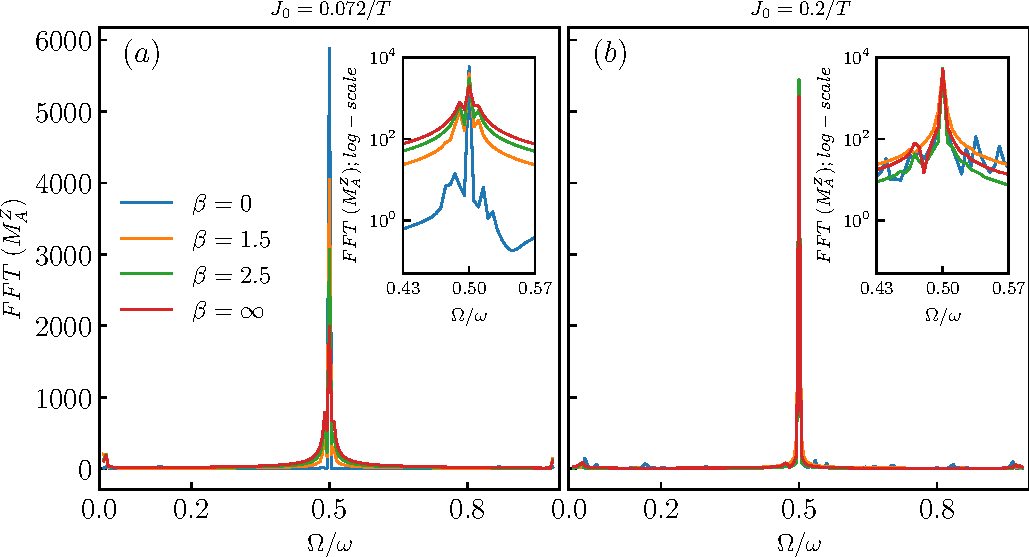
\includegraphics[width = 13cm]{figure10.pdf}
	\caption{
		Fast Fourier Transforms(FFT) of regional magnetization $M^z_{A}$ of the spin-chain. The magnetization of regions A are plotted as functions of time \sout{$(\omega/\omega_D)$}\red{$\Omega/\omega$} for both weak spin-coupling ($J_0=0.072/T$, left panel) and strong spin-coupling ($J_0=0.2/T$, right panels) and different ranges of spin interactions (characterized by $\beta$ as specified in the legends). The time period is fixed by setting drive parameters $h,\omega$ to the first CDT/DL point, \textit{i.e.} the first root of $\mathcal{J}_0(\chi)$. All other parameters are the same as the simulations visualized in figure~\ref{Fig:strong_weak_ea}. \red{In the inset the variation in FFT is plotted in logarithmic scale for small frequency window.}}
	\label{Fig:regionalFFT}
\end{figure}
The underlying mechanisms by which the DTC disintegrates can be investigated in frequency space by means of an FFT of regional magnetization.\todo{Explain why in strong coupling all -to -all DTC dissolves.} The results, obtained in a manner similar to the FFTs of the site magnetization in section~\ref{sec:level3}, are depicted in figure~\ref{Fig:regionalFFT}. In the regime of weak spin coupling, the subharmonic peaks at $\Omega=\omega/2$ exhibit a dominant influence on the continuum of frequency responses in $\Omega$. Consequently, this leads to a sustained regional magnetization over an extended period of time. As the parameter $\beta$ is strengthened,  the continuum of frequencies becomes more prominent, contributing to the faster disintegration of $M^Z_A$. In the scenario of strong coupling, the continuum is more prominent across all ranges, leading to a more rapid disintegration of the regional magnetization compared to the weak spin-coupling.

	
	
	\subsection{\label{sec:level41} Entanglement Entropy}
In contrast to the preceding subsection, which focused on the examination of macroscopic observables, the current section delves into a more direct analysis of microscopic aspects through the consideration of entanglement entropy (EE). The EE is commonly employed as a measure to quantify the degree of entanglement exhibited by quantum states across invariant subspaces. It provides valuable insight into quantum correlations and the ability to store information. The mathematical expression for the entanglement entropy, denoted $S_{AB}$, between areas A and B, can be described using the von-Neumann entropy~\cite{bayat_entanglement_2022,mendes-santos_measuring_2020}.   The density matrix of a pure state $\ket{\psi}$ is $\hat{\rho}= \ketbra{\psi}$. The reduced density matrices (RDMs) for regions A and B, denoted as $\hat{\rho}_A$ and $\hat{\rho}_B$ respectively, are obtained by taking the partial traces of $\hat{\rho}$ with respect to the complementary regions. Specifically, $\hat{\rho}_A$ is obtained by tracing out region B, \textit{i.e.}, $\hat{\rho}_A\equiv \Tr_B(\hat{\rho})$, while $\hat{\rho}_B\equiv\Tr_A(\hat{\rho})$. The entanglement entropy (EE) is determined by
\begin{equation} 
    S_{AB} = -\Tr\big[\hat{\rho}_A \ln\left(\hat{\rho}_A\right)\big] = -\Tr\big[\hat{\rho}_B \ln\left(\hat{\rho}_B\right)\big].
    \label{eq:vonentrop}
\end{equation}	
\begin{figure}[t!]
    \begin{center}
        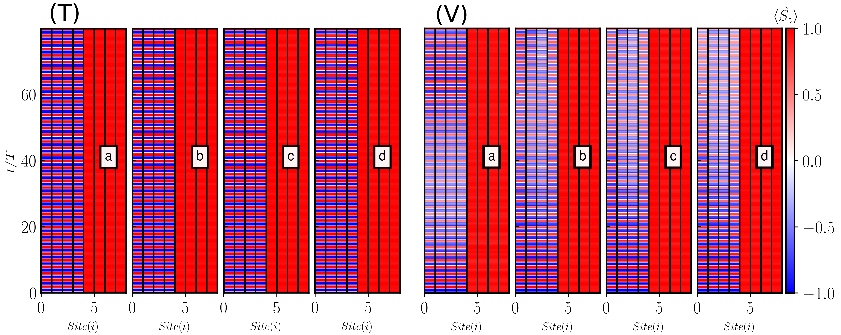
\includegraphics[width=10cm]{figure11.pdf}
    \end{center}
    \caption{Time evolution of Entanglement Entropy $S_{AB}$ between regions A and B as a function of time at the CDT/DL point. The left panel plot results for weak spin coupling, and the right panel plot results for stronger spin couplings. The corresponding values of $J_0$ are the same as those of figure~\ref{Fig:regiogionalmag}, and all other parameters are identical to previous simulations. The spin-spin coupling interaction in $\hat{H}_2$ during $T_2$ leads to the onset of an increase in EE. The growth rate of EE remains notably slow, persisting even up to $t=2000\;T$.}
    \label{Fig:entangle}
\end{figure}
We have extended previous simulations to  a later time point of $t=2000\;T$, and calculated the EE for  each time point. The results are plotted in figure~\ref{Fig:entangle} for both weak and strong spin coupling, while maintaining the driving parameters consistently at a CDT/DL point. The EE is found to start to rise from the onset of the first $T_2-cycle$, when spin interactions begin to impact the behavior of the spin chain. The increase in EE is observed to be gradual, even after prolonged interactions.  The EE exhibits a more rapid increase in the case of strong spin coupling compared to weak spin coupling. As evidenced by equation~\eqref{eq:floq_eff3}, the coupling present in the effective Hamiltonian is directly proportional to the rotational error $\epsilon_A$. When the value of $\epsilon_A$ is small, it effectively hinders the interaction between regions A and B, therefore suppressing the increase in EE. This corroborates the results depicted in figure~\ref{Fig:ea}, where the DTC appears to be more stable at smaller $\epsilon_A$ than at larger $\epsilon_A$.
	
When thermalized at infinite temperature, the EE is extensive and averages at $\displaystyle \overline{\expval{S_{AB}}}_T\rightarrow \left[N \ln{2}-1\right]/2$ \cite{Lu2021}. When localized, the EE per particle vanishes in the thermodynamic limit. For finite sizes, it can be approximated as $\overline{\expval{S_{AB}}}_L\approx \ln{2}$~\cite{sakurai_phys_nodate}. In our spin chain, $N=8$, yielding theoretical expressions, $\overline{\expval{S_{AB}}}_T\approx 2.27$, and $\overline{\expval{S_{AB}}}_L\approx 0.69$. The numerical values of the entanglement entropy (EE) are found to remain approximately in the range of $\in\left[0,0.6\right)$, as can be seen in figure~\ref{Fig:entangle}. This observation indicates that the entire system remains athermal and localized, even when a significant amount of time has elapsed.
\begin{figure}[t!]
	\begin{center}
		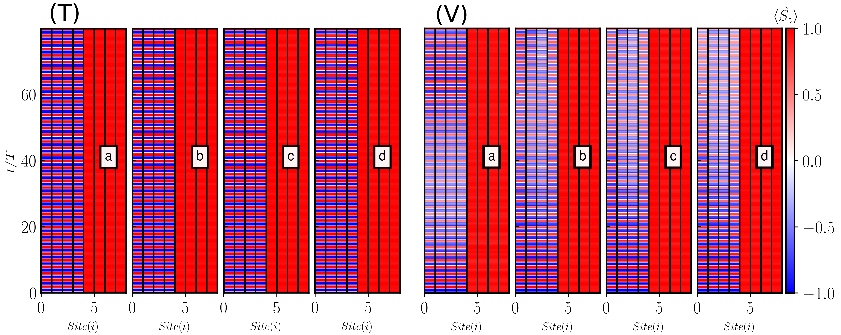
\includegraphics[width=15cm]{figure12.pdf}
	\end{center}
	\caption{Weak (left T- panels) and strong (right V-panels) additional static fields defined by $\gamma = J_0/5, J_0$ respectively ( where $J_0=0.2/T$ ), are applied in addition to the strong spin coupling and transverse field at different interaction ranges set by $\beta = 0.0$ (panels a), $\beta= 1.5$ (panels b), $\beta=2.5$ (panels c), and $\beta= \infty$ (panels d). The frequency of the drive is $\omega = 20$, amplitude $h$ is corresponding to CDT/DL point, $\epsilon_A=0.03$, $\epsilon_B=0.9$ and all other parameters are kept similar to previous simulations.  The local magnetization for each site (i) is plotted from $t=0$ to $t=80 T$.}
	\label{Fig:robustness}
\end{figure}	
\subsection{\label{sec:level43} Robustness against Static Fields}

The influence of the driving parameters $h, \omega$ significantly affects the long-lasting stability of the DTC-DMBL chimera. The stability of the chimera order diminishes even if there is a minor deviation from the CDT/DL point. This raises questions about the mechanisms by which the chimera resists external fields, even while functioning precisely at the CDT/DL point.
In order to conduct an investigation, we will now incorporate the static field $\hbar\hat{V}(\hat{\sigma}^{\gamma})$ discussed in section~\ref{sec:mdl_n_dynam} into the Hamiltonian $\hat{H}(t)$. This static field remains un-modulated by the pulses and acts on the system identically at all times. We conducted the simulation incorporating this field while all other parameters were maintained at the same values at CDT/DL point as in earlier simulations. 

We ran simulations for both strong ($\gamma=0.2/T$) and weak ($ \gamma= 0.2/5T$) field amplitudes. The findings are displayed in figure~\ref{Fig:robustness}. At low values of $\gamma$, the influence of spin interactions is more significant compared to the static field, leading to the continued existence of dynamical localization. Consequently, a stable chimera state of the DTC is observed. However, when the value of $\gamma$ increases, the static field becomes dominant over the interactions, resulting in the melting of the DTC after a few cycles. However, it is worth noting that the DMBL phase continues to exist even in the presence of the static field. Therefore, a chimera phase known as \textit{Thermal-DMBL} becomes apparent at longer time scales. Therefore, it is possible to achieve a strong DTC-DMBL chimera even when moderate external fields are present.
	
\section{\label{sec:level7} Summary and Conclusion}
A new quantum chimera state has been observed in a closed  system, where a discrete-time crystal (DTC) and a dynamically many-body localized (DMBL) phase coexist on a one-dimensional spin-$1/2$ chain. In order to achieve this, we have divided the lattice into two regions, labeled `A' and `B', based on their rotational errors ($\epsilon_{A/B}$). {We have applied two different Hamiltonians, modulated by a time-periodic square wave, which act on the spin chain at different times. One Hamiltonian conducts spin-flip operations only in region `A' during first duty-cycle of the square wave (for time $T_1$), while the other Hamiltonian induces global dynamical localization in the entire spin chain at the second duty cycle (for time $T_2$). This process repeats at every time-period of the square wave, resulting in the coexistence of a DTC phase in region A and a DMBL phase in region B.} We have applied specific high-frequency periodic drive parameters engineered to attain dynamical localization via Coherent Destruction of Tunneling (the CDT/DL point) during the $T_2$ cycle. We have produced the results of numerical simulations that have shown that the interaction on the spin chain plays an essential role in the formulation of the chimera and the stabilization of the DTC phase. Our results suggest that the DTC does not exhibit temporal persistence when the spin-spin coupling strength is weak. This was seen for all types of interaction ranges (except for all-to-all interactions). The presence of a strong spin coupling hinders the relaxation of spins away from the DTC, stabilizing the DTC phase regionally for long times throughout all interaction ranges. Interestingly, the stability of the DTC in region A is contingent on the stability of the DMBL phase in region B. The long-range spin interaction is very robust against the exchange energy per spin, and this enables the chimera to persist for both weak and strong coupling. 
The inter-region coupling term in the effective Floquet Hamiltonian in equation~\ref{eq:floq_eff3} is directly proportional to the spin rotation error $\epsilon_A$. We have tuned $\epsilon_A$ and found that the chimera can persist only if $\epsilon_A$ is small. In the case of larger values, there is an increased level of coupling between the two regions. This heightened coupling results in the immediate melting of the DTC for all interactions, except for long-range interactions.
	
To further study the resilience of this chimera against static perturbations, an additional external static field is included. Numerical simulations have demonstrated that the system is robust in the face of minor perturbations, as evidenced by the sustained presence of the DTC phase inside region A for an extended duration. However, when subjected to more significant perturbations, the robustness of the system diminishes, leading to rapid dissolution of the DTC phase across all spin-interaction types. The Floquet Hamiltonian, obtained analytically and supported by exact simulations, illustrates the coupling between regions A and B. The entanglement entropy rises at a very slow rate for both weak and strong regional spin interactions. Therefore, the entire system is effectively prevented from thermalizing. Additionally, the persistence of the DTC phase is directly dependent on the stability of the DMBL phase. Our proposed DTC-DMBL chimera model shows sustainability even at larger times.  With proper drive parametrization in other 1-dimensional spin models, such as the XY or XXZ models, DTC-DMBL can be realized. The experimental realization of this model and its dynamics can be achieved using trapped ions~\cite{sakurai_phys_nodate, Friedenauer2008}, as described in previous studies.
	
\ack{MR acknowledges The University of Burdwan for support through the State-Funded fellowship. AR acknowledges support from the University Grants Commission (UGC) of India, via BSR Startup Grant No. F.30-425/2018(BSR), also from the Science and Engineering Research Board (SERB, Govt. of India) Core Research Grant No. CRG/2018/004002. Additionally, AR thanks Prof. Tanmoy Banerjee, Dept. of Physics, The University of Burdwan, for useful discussions.}
\medskip

%Appendix
\clearpage

\appendix
\section{\label{sec:AppendixA} DMBL in $T_2$ time interval}

Let us consider a one-dimensional spin-$1/2$ chain consisting of $N$ spins, with Heisenberg exchange interaction between them. The interaction follows a power law decay rule, where the exchange energy between the $i^{th}$ and $j^{th}$ spins is presumed to be  $J_{ij}=J_0\abs{i-j}^{-\beta}$. Let us now  divide the chain into two regions, A and B by manipulating corresponding spin rotational errors, and introduce time dependencies via two pulse wave sequences in the manner described in section~\ref{sec:mdl_n_dynam} and figure~\ref{Fig:time_distribution}. The first sequence  induces spin-flips in region A within time $T_1$, and the second modulates a global sinusoidal periodic drive in the field \textit{s.t.} $h_D = -h\sin(\omega t)$ within time $T_2$, chosen to be such that the time period $T\equiv 2\pi/\omega = T_1 + T_2$ and $T_1 = T_2$. This drive parameters are controlled in such a way that the system is dynamically localized during the $T_2-$cycles.

The Hamiltonian during the $T_2-$cycle is $\displaystyle \hat{H}_2(t) = \hbar\sum_{i>j} J_{ij}\hat{\sigma}^y_i\hat{\sigma}^y_j - \hbar h \sin(\omega t) \sum_i \hat{\sigma}^z_i$. Let us define the free propagator 
\begin{equation}
    \hat{U}(t) \equiv \exp \bigg[-\frac{i}{\hbar}\int_{\frac{T}{2}}^{\frac{T}{2}+t} (-h \sin(\omega t'))dt' \hbar\sum_i\hat{\sigma}^z_i\bigg]
    =\prod_{i} \exp\big[-i \hat{\sigma}^z_i\zeta(t)\big],
\end{equation}
where, $\displaystyle \zeta (t) = h\int_{\frac{T}{2}}^{\frac{T}{2}+t}  (-\sin(\omega t')dt') =\frac{h}{\omega}(1-\cos(\omega t))$.
Now, the Hamiltonian can be transformed to the moving frame as follows \cite{haldar_statistical_2022}.
\begin{align}
    \hat{H^{mov}}(t) &= \hat{U}^\dagger(t) \hat{H}_2(t) \hat{U}(t)- i \hat{U}^\dagger(t) \partial_t \hat{U}(t) \nonumber\\
    &= \prod_{i} \exp\big[-i\hat{\sigma}^z_i \zeta(t)\big] \big[\hbar\sum_{ij}J_{ij}\hat{\sigma}^y_i\hat{\sigma}^y_j\big] \exp\big[ i\hat{\sigma}^z_i \zeta(t)\big]\nonumber\\
    &= \hbar\sum_{ij} J_{ij}\;\big[ e^{-i\hat{\sigma}^z_i \zeta(t)} \hat{\sigma}^y_i e^{i\hat{\sigma}^z_i \zeta(t)}\big]\quad \big[e^{-i\hat{\sigma}^z_j  \zeta(t)}\hat{\sigma}^y_j e^{i\hat{\sigma}^z_j \zeta(t)}\big]\nonumber\\
    &=\hbar\sum_{ij}J_{ij}\Big\{\hat{\sigma}^y_i\cos{\big[2\zeta(t)\big]}-\hat{\sigma}^x_i\sin{\big[2\zeta(t)\big]}\Big\}\Big\{\hat{\sigma}^y_j\cos{\big[2\zeta(t)\big]}-\hat{\sigma}^x_j\sin{\big[2\zeta(t)\big]}\Big\},\nonumber\\
    %&= \hbar\sum_{ij} J_{ij} \Big(\hat{\sigma}^y_i\hat{\sigma}^y_j\Big)e^{i2\hat{\sigma}^z_i \zeta(t)} e^{i2\hat{\sigma}^z_j \zeta(t)}\nonumber\\
    &= \hbar\sum_{ij} J_{ij}  \Big[ \hat{\sigma}^y_i\hat{\sigma}^y_j\cos^2(2\zeta) +\hat{\sigma}^x_i\hat{\sigma}^x_j \sin^2(2\zeta) - \frac12 (\sigma^y_i\hat{\sigma}^x_j + \hat{\sigma}^x_i\hat{\sigma}^y_j)\sin(4\zeta)\Big].
    \label{eq:hmovap1}
\end{align}
In the penultimate step, we used the Baker-Campbell-Hausdorff formula. Now, we invoke the Jacobi-Anger expansion, $e^{i\eta \cos(\theta)} = \sum_{n=-\infty}^{\infty}\mathcal{J}_n(\eta)e^{in\theta}$, where $\mathcal{J}_n(z)$ is the Bessel function of the first kind of $n^{th}$ order, and apply to the RHS of  equation~\ref{eq:hmovap1}. This produces a Fourier series expansion for each amplitude in
$\hat{H}^{mov}(t)$ with period $\omega$. In high frequency limit, where $\omega \gg J_0$, the Rotating Wave Approximation (RWA) allows for approximating the Fourier modes with their long time averages, thus removing the contributions of all fast-oscillating terms. This yields approximations
\begin{align}
\cos[2](2\zeta) &\approx \frac12 \Bigg[1+ \cos(\frac{4h}{\omega})\mathcal{J}_0\left(\frac{4h}{\omega}\right)\Bigg]\nonumber\\
\sin[2](2\zeta) &\approx \frac12 \Bigg[1- \cos(\frac{4h}{\omega})\mathcal{J}_0\left(\frac{4h}{\omega}\right)\Bigg]\nonumber\\
\sin(4\zeta)&\approx \frac12 \sin(\frac{4h}{\omega})\mathcal{J}_0\left(\frac{4h}{\omega}\right).
\label{eq:sqr}
\end{align}
Finally, we substitute the values from equation~\eqref{eq:sqr} into equation~\eqref{eq:hmovap1}. This reduces the moving frame Hamiltonian into a RWA-Hamiltonian ($\hat{H^{_{RWA}}}$) given below,
\begin{multline}
    \hat{H}^{mov}\approx \hat{H}^{_{RWA}} = \frac{\hbar}{2}\sum_{ij} J_{ij}  \Bigg\{ \hat{\sigma}^y_i\hat{\sigma}^y_j\Bigg[1+ \cos(\frac{4h}{\omega})\mathcal{J}_0\left(\frac{4h}{\omega}\right)\Bigg] +\hat{\sigma}^x_i\hat{\sigma}^x_j \Bigg[1- \cos(\frac{4h}{\omega})\mathcal{J}_0\left(\frac{4h}{\omega}\right)\Bigg] \\
    - \frac12 (\sigma^y_i\hat{\sigma}^x_j + \hat{\sigma}^x_i\hat{\sigma}^y_j)\sin(\frac{4h}{\omega})\mathcal{J}_0\left(\frac{4h}{\omega}\right)\Bigg\}.
    \label{eq:hrwa}
\end{multline}	
Now, for a particular $\omega$, if $h$ is controlled in such fashion that $\frac{4h}{\omega}$ lies on the CDT/DL point, given by a root of $\mathcal{J}_0\Big(\frac{4h}{\omega}\Big)$, then $\hat{H}^{_{RWA}}$ becomes the "CDT/DL Hamiltonian",
\begin{equation}
\hat{H}^{_{RWA}}_{_{CDT/DL}} = \frac{\hbar}{2}\sum_{ij} J_{ij}  \Big[\hat{\sigma}^x_i\hat{\sigma}^x_j + \hat{\sigma}^y_i\hat{\sigma}^y_j\Big].
\label{eq:hrwa:frz}
\end{equation}	
One limiting case of the $J_{ij}$s is the nearest-neighbor case, where $J_{ij} = J_0 \delta_{i\;j\pm1}$. In that case, performing a Jordan-Wigner Transformation ,
\begin{align}
\hat{\sigma}^x_i &= \left(\hat{c}_i + \hat{c}^\dagger_i\right) \prod_{j=0}^{i-1}\left(1-2\hat{c}^\dagger_j \hat{c}^{\;}_j\right),\nonumber\\
\hat{\sigma}^y_i &= i\left(\hat{c}_i - \hat{c}^\dagger_i\right) \prod_{j=0}^{i-1}\left(1-2\hat{c}^\dagger_j \hat{c}^{\;}_j\right),\nonumber\\
\hat{\sigma}^z_i &= 1-2\hat{c}^\dagger_i\hat{c}^{\;}_i,
\end{align}
maintains the locality of the Hamiltonian in the basis of fermion creation and annihilation operators $\hat{c}^{\;}_i, \hat{c}^\dagger_i$ \cite{Lieb1961, mbeng2020}. Here, the CDT/DL Hamiltonian transforms to the standard tight-binding Hamiltonian $\hat{H}^{_{RWA}}_{_{CDT/DL}}=(J_0/2)\sum_i \hat{c}^\dagger_i \hat{c}^{\;}_{i+1}$. The system is completely localized due to the presence of $N$ local (approximate) Noether Charges, given by $\hat{n}_m= \hat{d}^{\dagger}_m\hat{d}^{\;}_m$, where
\begin{equation}
\hat{d}_m = \frac{1}{\sqrt{N}}\sum_{n=0}^{N-1}e^{-\frac{2nm\pi i}{N}}\hat{c}_n.
\end{equation}
When the $J_{ij}$s are extended beyond the nearest-neighbour case to longer ranges, the locality of the Jordan Wigner transformation is destroyed. Nonetheless, the normal dynamics of the transverse field remains frozen at the CDT/DL point , since $\comm{H^{_{RWA}}_{_{CDT/DL}}}{\displaystyle\sum_i\sigma^z_i}=0$.

In our driving protocol, the system is always ideally populated in an eigenstate of the transverse field at the end of every $T_1$ time interval, with a $z-$polarized region A and a region B that is polarized in the opposite direction. Thus, the field dynamics will, in the ideal case, be frozen in all $T_2$ time intervals.

\section{\label{sec:AppendixB} Effective Floquet Hamiltonian}

Floquet theory is a widely used methodology for evaluating the dynamical behavior of time-periodic systems.  In a quantum system that is time periodic with period $T$, the Hamiltonian obeys $\hat{H}(t+T) = \hat{H}(t)\;\forall t$. If we split the time-dependent part from the time-independent, or \textit{d.c.} part, we can write
\begin{equation*}
    \hat{H}(t) = \hat{H}_0 + \varepsilon \hat{H}_1(t)
\end{equation*}
The corresponding propagator can be obtained by solving the Schr\"odinger equation $\displaystyle{i\hbar \partial_t \hat{U}(t) = \hat{H}(t) \hat{U}(t)}$.  The propagator at $t=T$, given by $ \hat{\mathcal{F}}\equiv \hat{U}(T)$ is called the \textit{Floquet operator}. Now, it follows from Floquet's Theorem that, if the system is strobed at integer multiples of $T$, the dynamics can be mapped to that of a time-independent effective Hamiltonian $\hat{H}_F$, such that  $\displaystyle\hat{U}(nT) = \exp\bigg[-\frac{i}{\hbar}\hat{H}_F\; nT \bigg]$~\cite{Eckardt_2015}.  The operator$\hat{H}_F$ (also denoted by $H^\mathrm{eff}$) is obtained from the original time-dependent Hamiltonian, and is given by, $\displaystyle \hat{H}_F = \Bigg(\hat{H}(t) - i\hbar \pdv{t}\Bigg)$ evaluated at $t=T$. 


Now, the proposed spin chain in equation~\eqref{eq:cleanham} needs to evolve for at least two time periods to manifest a DTC. If the effective time-independent Hamiltonian at that time is denoted by $\hat{H}^{\mathrm{eff}}_{\epsilon_A, 2T}$, then, the propagator
\begin{align}
    \hat{\mathcal{F}}^{2} &\equiv \exp\Big(-\frac{i}{\hbar}\hat{H}_{\epsilon_A, 2T}^{\mathrm{eff}}\;2T\Big) \label{eq:heff}\\ 
    &= \mathcal{T}\exp\Big(-\frac{i}{\hbar}\int_{\frac{3T}{2}}^{2T}\hat{H}_2(t) dt\Big)
    \exp\Big(-\frac{i}{\hbar}\hat{H}_1T_1\Big)\nonumber\\
    & \hskip 5cm \mathcal{T}\exp\Big(-\frac{i}{\hbar}\int_{\frac{T}{2}}^{T}\hat{H}_2(t) dt\Big)\exp\Big(-\frac{i}{\hbar}\hat{H}_1T_1\Big).
    \label{eq:2tprop}
\end{align}
Here $\mathcal{T}$ denotes the time-ordering operation. 
To evaluate $\hat{\mathcal{F}}^2$, we start by calculating each of the four terms in RHS of equation~\ref{eq:2tprop}. During the $T_1-$cycle, $t\in[0,T/2]$, and the time-independent Hamiltonian $\hat{H}_1$ is applied on spin chain. Thus,
\begin{equation}
    \exp\Big(-\frac{i}{\hbar} \hat{H}_1 T_1\Big) = 	\exp\Bigg[\frac{-i(1-\epsilon_A)\pi}{2}\sum_{l \in A}\hat{\sigma}^x_l\Bigg].
    \label{eq:effham1}
\end{equation}	
It is evident that the effective Hamiltonian for $t \in[T, 3T/2]$ will be same as that obtained from equation~\eqref{eq:effham1}. Next, during the $T_2-$cycle, $t\in[T/2,T]$, and the time-dependent Hamiltonian, $\hat{H_2}(t)$ is applied. Therefore,
\begin{align}
    \mathcal{T}\exp\Big(-\frac{i}{\hbar}\int_{\frac{T}{2}}^{T}\hat{H}_2(t) dt\Big) &= \exp( -\frac{i}{\hbar}\int_{\frac{T}{2}}^{T}\Big[\hbar\sum_{i\neq j}J_{ij}\hat{\sigma}^y_i\hat{\sigma}^y_j-\hbar h\sin(\omega t)\sum_i\hat{\sigma}^z_i\Big] dt)\nonumber\\
    &= \exp(-i \Big[\sum_{i\neq j}J_{ij}\hat{\sigma}^y_i\hat{\sigma}^y_j \frac{T}{2} + \frac{2h}{\omega}\sum_i \sigma^z_i\Big])
    \label{eq:t2hamilt}
\end{align}
Clearly, the effective Hamiltonian for the times  $t \in[3T/2, 2T]$ will also be the same as equation~\eqref{eq:t2hamilt}. Now,	let us consider the case where $\epsilon_A \neq 0$ and $\epsilon_B=1$. Furthermore, let us define the operators $\displaystyle \hat{V}_{\epsilon_A} \equiv \exp\Big(\frac{i\epsilon_A \pi}{2}\sum_{l\in A}\hat{\sigma}^x_l\Big), \displaystyle \hat{\theta}_l \equiv 2 \left(\sum_{m \in B}J_{lm}\hat{\sigma}^y_m \frac{T}{2} \right)$; the latter describes a rotation acting on operator $\hat{\sigma}^y_l$ in only region B.  Now, we can expand expression for the  $T_2-$cycle propagator in equation~\ref{eq:t2hamilt} by splitting the contributions from regions A and B. This yields
\begin{multline}
    \mathcal{T}\exp\bigg\{-\frac{i}{\hbar}\int_{\frac{T}{2}}^{T} \hat{H}_2(t) dt\bigg\} = \exp\Bigg\{-i \bigg[ \sum_{l,m\in A}J_{lm} \hat{\sigma}_l^y\hat{\sigma}_m^y +\sum_{l,m\in B}J_{lm}
    \hat{\sigma_l^y}\hat{\sigma_m^y}+\sum_{\substack{%
            l \in A,\\
            m \in B\hfill}} J_{lm}\hat{\sigma}^y_l\hat{\sigma}^y_m\\
    +\frac{4h}{\omega T}\big( \sum_{l\in A}^{}\hat{\sigma}^z_l + \sum_{m\in B}^{}\hat{\sigma}^z_m\big)\bigg]\frac{T}{2}\Bigg\}.
    \label{eq:effham3}
\end{multline}	
Substituting the RHS of equations~\eqref{eq:effham1} \& \eqref{eq:effham3} into the RHS of equation~\eqref{eq:2tprop} yields    	
\begin{multline}
    \hat{\mathcal{F}}^2 
    = \exp\Bigg\{-i \Bigg[ \sum_{l,m\in A}J_{lm} \hat{\sigma}^y_l\hat{\sigma}^y_m\frac{T}{2} +\sum_{l,m\in B}J_{lm} \hat{\sigma}^y_l\hat{\sigma}^y_m\frac{T}{2}+\sum_{\substack{%
            l \in A,\\
            m \in B\hfill}} J_{lm}\hat{\sigma}^y_l\hat{\sigma}^y_m\frac{T}{2} \\
            +\frac{2h}{\omega }\left( +\sum_{l\in A}^{}\hat{\sigma}^z_l + \sum_{m\in B}^{}\hat{\sigma}^z_m\right)\Bigg]\Bigg\} \hat{V}_{\epsilon_A} \exp\Bigg\{-i \Bigg[ \sum_{l,m\in A}J_{lm} \hat{\sigma}^y_l\hat{\sigma}^y_m\frac{T}{2}\\ +\sum_{l,m\in B}J_{lm} \hat{\sigma}^y_l\hat{\sigma}^y_m\frac{T}{2}
            -\sum_{\substack{%
            l \in A,\\
            m \in B\hfill}} J_{lm}\hat{\sigma}^y_l\hat{\sigma}^y_m\frac{T}{2} +\frac{2h}{\omega}\left( -\sum_{l\in A}^{}\hat{\sigma}^z_l + \sum_{m\in B}^{}\hat{\sigma}^z_m\right)\Bigg]\Bigg\} \hat{V}_{\epsilon_A}.\nonumber
\end{multline}
We can simplify this expression further with the Suzuki–Trotter decomposition\cite{Ostmeyer_2023, Hatano2005} that all operators with norms $\mathcal{O}(T^2)$ can be neglected in comparison to those with norm $\sim T$ for sufficiently large $\omega\equiv 2\pi/T$. Thus, for instance, $e^{T\hat{A} + T\hat{B}}= e^{T\hat{A}}\; e^{T\hat{B}}\;e^{C_2 T^2\left[\hat{A}, \hat{B}\right]}\;e^{C_3 T^3\left[\hat{A},\left[\hat{A}, \hat{B}\right]\right]}\;\dots \approx e^{T\hat{A}} e^{T\hat{B}}$, once all higher order operators are neglected after applying the Zassenhaus' formula~\cite{Magnus1954}. This yields
\begin{multline}	
    \hat{\mathcal{F}}^2 	\approx\exp\Bigg[-i \sum_{l,m\in A}J_{lm} \hat{\sigma}^y_l\hat{\sigma}^y_m\frac{T}{2}\Bigg] \exp\Bigg[-i\left(\frac{2h}{\omega } \sum_{l\in A}^{}\hat{\sigma}^z_l + \sum_{l \in A}\frac{\hat{\theta}_{l}}{2}\hat{\sigma}^y_l\right)\Bigg] 
    \hat{V}_{\epsilon_A} \\
    \exp\Bigg[i \left(\sum_{l \in A}\frac{\hat{\theta}_{l}}{2}\hat{\sigma}^y_l + \frac{2h}{\omega} \sum_{l\in A}^{}\hat{\sigma}^z_l\right)\Bigg] \exp\Bigg[-i\sum_{l,m\in A}J_{lm} \hat{\sigma}^y_l\hat{\sigma}^y_m\frac{T}{2}\Bigg] \exp\big[-i H_B T\big]\hat{V}_{\epsilon_A},\nonumber
\end{multline}
where, for the sake of brevity, we have defined the $T_2-$cycle Hamiltonian in region-B, $\displaystyle {H}_B \equiv \sum_{l,m\in B} J_{lm} \hat{\sigma}^y_l\hat{\sigma}^y_m + \frac{4h}{\omega T}\sum_{m \in B}\hat{\sigma^z_m}$. We now observe that $\hat{\theta}_l$ commutes with all operators that live in region$-A$, thus allowing us to temporarily treat it as a $c-$number in algebraic manipulations, allowing for the simplification
\begin{align}		
    \hat{\mathcal{F}}^2 	\approx& \exp\Bigg[-2i  \sum_{l,m\in A}J_{lm} \hat{\sigma}^y_l\hat{\sigma}^y_m\frac{T}{2}\Bigg]\exp\Bigg[\frac{i \epsilon_A \pi}{2}\sum_{l\in A}\Bigg\{\hat{\sigma}^x_l \cos(\hat{\theta}_l)\cos(\frac{4h}{\omega})\nonumber\\
    &+ \hat{\sigma}^y_l \cos(\hat{\theta}_l)\sin(\frac{4h}{\omega})-\hat{\sigma}^z_l \sin(\hat{\theta}_l)\Bigg\}\Bigg] \exp\big[-i H_B T\big]\hat{V}_{\epsilon_A}\nonumber\\
    =&\exp\Bigg[-2i \sum_{l,m\in A}J_{lm} \hat{\sigma}_l^y\hat{\sigma}_m^y\frac{T}{2}\Bigg] \exp\Big(\frac{i\epsilon_A \pi}{2}\sum_{l\in A}\hat{\sigma^x_l}\Big) \exp\Bigg[\frac{i \epsilon_A \pi}{2}\sum_{l\in A}\Bigg\{\hat{\sigma}^x_l \cos(\hat{\theta}_l)\nonumber\\
    & \cos(\frac{4h}{\omega})+\hat{\sigma}^y_l \cos(\hat{\theta}_l)\sin(\frac{4h}{\omega})-\hat{\sigma}^z_l \sin(\hat{\theta}_l)\Bigg\}\Bigg]\exp\big[-i H_B T\big]\nonumber\\
    =&\exp\Bigg[-2i\sum_{l,m\in A}J_{lm}\hat{\sigma}^y_l\hat{\sigma}^y_m \frac{T}{2}\Bigg] \exp\Bigg[-i\epsilon_A \pi \sum_{\substack{l,m \in A\\l\neq m}}J_{lm} \hat{\sigma}^z_l\hat{\sigma}^y_m\frac{T}{2}\Bigg] 
     \exp\Bigg[\frac{i \epsilon_A \pi}{2}\sum_{l\in A}\Bigg\{\hat{\sigma}^x_l\nonumber\\
     &\Bigg(1+ \cos(\hat{\theta}_l)\cos(\frac{4h}{\omega})\Bigg)
    +\hat{\sigma}^y_l \cos(\hat{\theta}_l)\sin(\frac{4h}{\omega})-\hat{\sigma}^z_l \sin(\hat{\theta}_l)\Bigg\}\Bigg] \exp\big[-i H_B T\big].
\end{align}
Next, we apply the Baker-Campbell-Hausdorff formula~\cite{Magnus1954} successively to all pairs of exponents in the RHS, neglecting all operators with norms $\mathcal{O}(T^2)$ as before, followed by substitution into the RHS of equation~\ref{eq:2tprop}. Finally, substitution into equation~\ref{eq:heff} yields the effective Floquet Hamiltonian in the high-frequency limit, 
\begin{multline}
    H^{\mathrm{eff}} \approx\frac{\hbar}{2} \sum_{l,m\in A}J_{lm}\hat{\sigma}_l^y\hat{\sigma}_m^y +\frac{\hbar \epsilon_A \pi}{4} \sum_{\substack{l,m\in A\\l\neq m}} J_{lm}\hat{\sigma}^z_l\hat{\sigma}^y_m + \frac{\hbar}{2}\sum_{l,m\in B}J_{lm}\hat{\sigma}_l^y \hat{\sigma}_m^y + \frac{h\hbar}{\pi}\sum_{m \in B}\hat{\sigma}^z_m \\ -\frac{\hbar \pi \epsilon_A}{4T}\sum_{l\in A}\Bigg\{\hat{\sigma}^x_l \bigg[\cos(\hat{\theta}_l)\cos(\frac{4h}{\omega})+1 \bigg] + \hat{\sigma}^y_l \cos(\hat{\theta}_l)\sin(\frac{4h}{\omega})-\hat{\sigma}^z_l \sin(\hat{\theta}_l)\Bigg\}.
    \label{eq:app:nfloq_eff3}
\end{multline}
In the limit of very high frequencies, $T\rightarrow 0$, leading to asymptotically vanishing $\hat{\theta}_l$. In this limit, the coupling between regions manifests as effective fields $\sim \hat{\sigma}^{x,y}_l$ in region $A$ whose intensities depend only on $\epsilon_A$, and the ratio $\frac{4h}{\omega}$. When $h$ is set to an odd multiple of $\pi\omega/4$, these effective fields vanish in the asymptotic limit, causing the regions $A$ and $B$ to decouple completely.

% Bibliography
\bibliographystyle{iopart-num}
\bibliography{chimera}
\end{document}
